% Options for packages loaded elsewhere
\PassOptionsToPackage{unicode}{hyperref}
\PassOptionsToPackage{hyphens}{url}
\PassOptionsToPackage{dvipsnames,svgnames,x11names}{xcolor}
%
\documentclass[
  12pt,
  letterpaper,
]{book}

\usepackage{amsmath,amssymb}
\usepackage{iftex}
\ifPDFTeX
  \usepackage[T1]{fontenc}
  \usepackage[utf8]{inputenc}
  \usepackage{textcomp} % provide euro and other symbols
\else % if luatex or xetex
  \usepackage{unicode-math}
  \defaultfontfeatures{Scale=MatchLowercase}
  \defaultfontfeatures[\rmfamily]{Ligatures=TeX,Scale=1}
\fi
\usepackage{lmodern}
\ifPDFTeX\else  
    % xetex/luatex font selection
\fi
% Use upquote if available, for straight quotes in verbatim environments
\IfFileExists{upquote.sty}{\usepackage{upquote}}{}
\IfFileExists{microtype.sty}{% use microtype if available
  \usepackage[]{microtype}
  \UseMicrotypeSet[protrusion]{basicmath} % disable protrusion for tt fonts
}{}
\makeatletter
\@ifundefined{KOMAClassName}{% if non-KOMA class
  \IfFileExists{parskip.sty}{%
    \usepackage{parskip}
  }{% else
    \setlength{\parindent}{0pt}
    \setlength{\parskip}{6pt plus 2pt minus 1pt}}
}{% if KOMA class
  \KOMAoptions{parskip=half}}
\makeatother
\usepackage{xcolor}
\usepackage[margin=1in]{geometry}
\setlength{\emergencystretch}{3em} % prevent overfull lines
\setcounter{secnumdepth}{5}
% Make \paragraph and \subparagraph free-standing
\makeatletter
\ifx\paragraph\undefined\else
  \let\oldparagraph\paragraph
  \renewcommand{\paragraph}{
    \@ifstar
      \xxxParagraphStar
      \xxxParagraphNoStar
  }
  \newcommand{\xxxParagraphStar}[1]{\oldparagraph*{#1}\mbox{}}
  \newcommand{\xxxParagraphNoStar}[1]{\oldparagraph{#1}\mbox{}}
\fi
\ifx\subparagraph\undefined\else
  \let\oldsubparagraph\subparagraph
  \renewcommand{\subparagraph}{
    \@ifstar
      \xxxSubParagraphStar
      \xxxSubParagraphNoStar
  }
  \newcommand{\xxxSubParagraphStar}[1]{\oldsubparagraph*{#1}\mbox{}}
  \newcommand{\xxxSubParagraphNoStar}[1]{\oldsubparagraph{#1}\mbox{}}
\fi
\makeatother

\usepackage{color}
\usepackage{fancyvrb}
\newcommand{\VerbBar}{|}
\newcommand{\VERB}{\Verb[commandchars=\\\{\}]}
\DefineVerbatimEnvironment{Highlighting}{Verbatim}{commandchars=\\\{\}}
% Add ',fontsize=\small' for more characters per line
\usepackage{framed}
\definecolor{shadecolor}{RGB}{241,243,245}
\newenvironment{Shaded}{\begin{snugshade}}{\end{snugshade}}
\newcommand{\AlertTok}[1]{\textcolor[rgb]{0.68,0.00,0.00}{#1}}
\newcommand{\AnnotationTok}[1]{\textcolor[rgb]{0.37,0.37,0.37}{#1}}
\newcommand{\AttributeTok}[1]{\textcolor[rgb]{0.40,0.45,0.13}{#1}}
\newcommand{\BaseNTok}[1]{\textcolor[rgb]{0.68,0.00,0.00}{#1}}
\newcommand{\BuiltInTok}[1]{\textcolor[rgb]{0.00,0.23,0.31}{#1}}
\newcommand{\CharTok}[1]{\textcolor[rgb]{0.13,0.47,0.30}{#1}}
\newcommand{\CommentTok}[1]{\textcolor[rgb]{0.37,0.37,0.37}{#1}}
\newcommand{\CommentVarTok}[1]{\textcolor[rgb]{0.37,0.37,0.37}{\textit{#1}}}
\newcommand{\ConstantTok}[1]{\textcolor[rgb]{0.56,0.35,0.01}{#1}}
\newcommand{\ControlFlowTok}[1]{\textcolor[rgb]{0.00,0.23,0.31}{\textbf{#1}}}
\newcommand{\DataTypeTok}[1]{\textcolor[rgb]{0.68,0.00,0.00}{#1}}
\newcommand{\DecValTok}[1]{\textcolor[rgb]{0.68,0.00,0.00}{#1}}
\newcommand{\DocumentationTok}[1]{\textcolor[rgb]{0.37,0.37,0.37}{\textit{#1}}}
\newcommand{\ErrorTok}[1]{\textcolor[rgb]{0.68,0.00,0.00}{#1}}
\newcommand{\ExtensionTok}[1]{\textcolor[rgb]{0.00,0.23,0.31}{#1}}
\newcommand{\FloatTok}[1]{\textcolor[rgb]{0.68,0.00,0.00}{#1}}
\newcommand{\FunctionTok}[1]{\textcolor[rgb]{0.28,0.35,0.67}{#1}}
\newcommand{\ImportTok}[1]{\textcolor[rgb]{0.00,0.46,0.62}{#1}}
\newcommand{\InformationTok}[1]{\textcolor[rgb]{0.37,0.37,0.37}{#1}}
\newcommand{\KeywordTok}[1]{\textcolor[rgb]{0.00,0.23,0.31}{\textbf{#1}}}
\newcommand{\NormalTok}[1]{\textcolor[rgb]{0.00,0.23,0.31}{#1}}
\newcommand{\OperatorTok}[1]{\textcolor[rgb]{0.37,0.37,0.37}{#1}}
\newcommand{\OtherTok}[1]{\textcolor[rgb]{0.00,0.23,0.31}{#1}}
\newcommand{\PreprocessorTok}[1]{\textcolor[rgb]{0.68,0.00,0.00}{#1}}
\newcommand{\RegionMarkerTok}[1]{\textcolor[rgb]{0.00,0.23,0.31}{#1}}
\newcommand{\SpecialCharTok}[1]{\textcolor[rgb]{0.37,0.37,0.37}{#1}}
\newcommand{\SpecialStringTok}[1]{\textcolor[rgb]{0.13,0.47,0.30}{#1}}
\newcommand{\StringTok}[1]{\textcolor[rgb]{0.13,0.47,0.30}{#1}}
\newcommand{\VariableTok}[1]{\textcolor[rgb]{0.07,0.07,0.07}{#1}}
\newcommand{\VerbatimStringTok}[1]{\textcolor[rgb]{0.13,0.47,0.30}{#1}}
\newcommand{\WarningTok}[1]{\textcolor[rgb]{0.37,0.37,0.37}{\textit{#1}}}

\providecommand{\tightlist}{%
  \setlength{\itemsep}{0pt}\setlength{\parskip}{0pt}}\usepackage{longtable,booktabs,array}
\usepackage{calc} % for calculating minipage widths
% Correct order of tables after \paragraph or \subparagraph
\usepackage{etoolbox}
\makeatletter
\patchcmd\longtable{\par}{\if@noskipsec\mbox{}\fi\par}{}{}
\makeatother
% Allow footnotes in longtable head/foot
\IfFileExists{footnotehyper.sty}{\usepackage{footnotehyper}}{\usepackage{footnote}}
\makesavenoteenv{longtable}
\usepackage{graphicx}
\makeatletter
\def\maxwidth{\ifdim\Gin@nat@width>\linewidth\linewidth\else\Gin@nat@width\fi}
\def\maxheight{\ifdim\Gin@nat@height>\textheight\textheight\else\Gin@nat@height\fi}
\makeatother
% Scale images if necessary, so that they will not overflow the page
% margins by default, and it is still possible to overwrite the defaults
% using explicit options in \includegraphics[width, height, ...]{}
\setkeys{Gin}{width=\maxwidth,height=\maxheight,keepaspectratio}
% Set default figure placement to htbp
\makeatletter
\def\fps@figure{htbp}
\makeatother
% definitions for citeproc citations
\NewDocumentCommand\citeproctext{}{}
\NewDocumentCommand\citeproc{mm}{%
  \begingroup\def\citeproctext{#2}\cite{#1}\endgroup}
\makeatletter
 % allow citations to break across lines
 \let\@cite@ofmt\@firstofone
 % avoid brackets around text for \cite:
 \def\@biblabel#1{}
 \def\@cite#1#2{{#1\if@tempswa , #2\fi}}
\makeatother
\newlength{\cslhangindent}
\setlength{\cslhangindent}{1.5em}
\newlength{\csllabelwidth}
\setlength{\csllabelwidth}{3em}
\newenvironment{CSLReferences}[2] % #1 hanging-indent, #2 entry-spacing
 {\begin{list}{}{%
  \setlength{\itemindent}{0pt}
  \setlength{\leftmargin}{0pt}
  \setlength{\parsep}{0pt}
  % turn on hanging indent if param 1 is 1
  \ifodd #1
   \setlength{\leftmargin}{\cslhangindent}
   \setlength{\itemindent}{-1\cslhangindent}
  \fi
  % set entry spacing
  \setlength{\itemsep}{#2\baselineskip}}}
 {\end{list}}
\usepackage{calc}
\newcommand{\CSLBlock}[1]{\hfill\break\parbox[t]{\linewidth}{\strut\ignorespaces#1\strut}}
\newcommand{\CSLLeftMargin}[1]{\parbox[t]{\csllabelwidth}{\strut#1\strut}}
\newcommand{\CSLRightInline}[1]{\parbox[t]{\linewidth - \csllabelwidth}{\strut#1\strut}}
\newcommand{\CSLIndent}[1]{\hspace{\cslhangindent}#1}

% header.tex
\usepackage{xcolor}        % Para colores
\usepackage{polyglossia}   % Soporte de idiomas con XeLaTeX
\setdefaultlanguage{spanish}

% Definición de colores personalizados
\definecolor{fecundidad}{HTML}{FFC125}      % Amarillo
\definecolor{supervivencia}{HTML}{36648B}   % Azul
\definecolor{crecimiento}{HTML}{548B54}     % Verde
\definecolor{retroceso}{HTML}{7A378B}       % Violeta
\definecolor{permanencia}{HTML}{26466A}     % Azul oscuro
\usepackage{booktabs}
\usepackage{caption}
\usepackage{longtable}
\usepackage{colortbl}
\usepackage{array}
\usepackage{anyfontsize}
\usepackage{multirow}
\makeatletter
\@ifpackageloaded{caption}{}{\usepackage{caption}}
\AtBeginDocument{%
\ifdefined\contentsname
  \renewcommand*\contentsname{Table of contents}
\else
  \newcommand\contentsname{Table of contents}
\fi
\ifdefined\listfigurename
  \renewcommand*\listfigurename{List of Figures}
\else
  \newcommand\listfigurename{List of Figures}
\fi
\ifdefined\listtablename
  \renewcommand*\listtablename{List of Tables}
\else
  \newcommand\listtablename{List of Tables}
\fi
\ifdefined\figurename
  \renewcommand*\figurename{Figure}
\else
  \newcommand\figurename{Figure}
\fi
\ifdefined\tablename
  \renewcommand*\tablename{Table}
\else
  \newcommand\tablename{Table}
\fi
}
\@ifpackageloaded{float}{}{\usepackage{float}}
\floatstyle{ruled}
\@ifundefined{c@chapter}{\newfloat{codelisting}{h}{lop}}{\newfloat{codelisting}{h}{lop}[chapter]}
\floatname{codelisting}{Listing}
\newcommand*\listoflistings{\listof{codelisting}{List of Listings}}
\makeatother
\makeatletter
\makeatother
\makeatletter
\@ifpackageloaded{caption}{}{\usepackage{caption}}
\@ifpackageloaded{subcaption}{}{\usepackage{subcaption}}
\makeatother

\ifLuaTeX
  \usepackage{selnolig}  % disable illegal ligatures
\fi
\usepackage{bookmark}

\IfFileExists{xurl.sty}{\usepackage{xurl}}{} % add URL line breaks if available
\urlstyle{same} % disable monospaced font for URLs
\hypersetup{
  colorlinks=true,
  linkcolor={Maroon},
  filecolor={Maroon},
  citecolor={Blue},
  urlcolor={Blue},
  pdfcreator={LaTeX via pandoc}}


\author{}
\date{}

\begin{document}
\frontmatter

\renewcommand*\contentsname{Table of contents}
{
\hypersetup{linkcolor=}
\setcounter{tocdepth}{2}
\tableofcontents
}

\mainmatter
\chapter{Acercamiento Bayesiano para calcular transiciones y
fertilidades}\label{acercamiento-bayesiano-para-calcular-transiciones-y-fertilidades}

Por: Raymond L. Tremblay

\begin{Shaded}
\begin{Highlighting}[]
\ControlFlowTok{if}\NormalTok{ (}\SpecialCharTok{!}\FunctionTok{require}\NormalTok{(}\StringTok{"pacman"}\NormalTok{)) }\FunctionTok{install.packages}\NormalTok{(}\StringTok{"pacman"}\NormalTok{)}
\NormalTok{pacman}\SpecialCharTok{::}\FunctionTok{p\_load}\NormalTok{(janitor, tidyverse, devtools)}

\FunctionTok{library}\NormalTok{(tidyverse)}
\FunctionTok{library}\NormalTok{(janitor)}
\FunctionTok{library}\NormalTok{(popbio) }\CommentTok{\# para la función projection.matrix()}
\FunctionTok{library}\NormalTok{(devtools) }\CommentTok{\# para instalar el paquete desde github}
\FunctionTok{library}\NormalTok{(raretrans) }\CommentTok{\# vea abajo para instalar esta libreria}
\FunctionTok{library}\NormalTok{(DiagrammeR)}
\FunctionTok{library}\NormalTok{(Rage)}
\FunctionTok{library}\NormalTok{(gt)}
\end{Highlighting}
\end{Shaded}

\begin{Shaded}
\begin{Highlighting}[]
\NormalTok{rlt\_theme }\OtherTok{\textless{}{-}} \FunctionTok{theme}\NormalTok{(}
  \AttributeTok{axis.title.y =} \FunctionTok{element\_text}\NormalTok{(}\AttributeTok{colour =} \StringTok{"grey20"}\NormalTok{, }\AttributeTok{size =} \DecValTok{10}\NormalTok{, }\AttributeTok{face =} \StringTok{"bold"}\NormalTok{),}
  \AttributeTok{axis.text.x =} \FunctionTok{element\_text}\NormalTok{(}\AttributeTok{colour =} \StringTok{"grey20"}\NormalTok{, }\AttributeTok{size =} \DecValTok{10}\NormalTok{, }\AttributeTok{face =} \StringTok{"bold"}\NormalTok{),}
  \AttributeTok{axis.text.y =} \FunctionTok{element\_text}\NormalTok{(}\AttributeTok{colour =} \StringTok{"grey20"}\NormalTok{, }\AttributeTok{size =} \DecValTok{15}\NormalTok{, }\AttributeTok{face =} \StringTok{"bold"}\NormalTok{),}
  \AttributeTok{axis.title.x =} \FunctionTok{element\_text}\NormalTok{(}\AttributeTok{colour =} \StringTok{"grey20"}\NormalTok{, }\AttributeTok{size =} \DecValTok{15}\NormalTok{, }\AttributeTok{face =} \StringTok{"bold"}\NormalTok{)}
\NormalTok{) }\SpecialCharTok{+}
  \FunctionTok{theme}\NormalTok{(}
    \CommentTok{\# Remover los border}
    \AttributeTok{panel.border =} \FunctionTok{element\_blank}\NormalTok{(),}
    \CommentTok{\# Remover las lineas}
    \AttributeTok{panel.grid.major =} \FunctionTok{element\_blank}\NormalTok{(),}
    \AttributeTok{panel.grid.minor =} \FunctionTok{element\_blank}\NormalTok{(),}
    \CommentTok{\# Remove el fondo del panel}
    \AttributeTok{panel.background =} \FunctionTok{element\_blank}\NormalTok{(),}
    \CommentTok{\# añadir lineas más gruesas}
    \AttributeTok{axis.line.x =} \FunctionTok{element\_line}\NormalTok{(}\AttributeTok{colour =} \StringTok{"black"}\NormalTok{, }\AttributeTok{linewidth =} \DecValTok{1}\NormalTok{),}
    \AttributeTok{axis.line.y =} \FunctionTok{element\_line}\NormalTok{(}\AttributeTok{colour =} \StringTok{"black"}\NormalTok{, }\AttributeTok{linewidth =} \DecValTok{1}\NormalTok{)}
\NormalTok{  )}


\NormalTok{diverging}\OtherTok{=} \FunctionTok{c}\NormalTok{(}\StringTok{"\#009392"}\NormalTok{,}\StringTok{"\#CF597E"}\NormalTok{,}\StringTok{"\#E9E29C"}\NormalTok{, }\StringTok{"\#39B185"}\NormalTok{,}\StringTok{"\#EEB479"}\NormalTok{ , }\StringTok{"\#9CCB86"}\NormalTok{ )}


\CommentTok{\# {-}{-}{-} 2. Combine them into a list object {-}{-}{-}}
\CommentTok{\# This list can be added to the plot with a single \textquotesingle{}+\textquotesingle{}}
\NormalTok{rlt\_style\_fill }\OtherTok{\textless{}{-}} \ControlFlowTok{function}\NormalTok{() \{}
  \FunctionTok{list}\NormalTok{(}
\NormalTok{    rlt\_theme,}
    \FunctionTok{scale\_fill\_manual}\NormalTok{(}\AttributeTok{values =}\NormalTok{ diverging)}
\NormalTok{  )}
\NormalTok{\}}


\NormalTok{rlt\_style\_colour }\OtherTok{\textless{}{-}} \ControlFlowTok{function}\NormalTok{() \{}
  \FunctionTok{list}\NormalTok{(}
\NormalTok{    rlt\_theme,}
    \FunctionTok{scale\_colour\_manual}\NormalTok{(}\AttributeTok{values =}\NormalTok{ diverging)}
\NormalTok{  )}
\NormalTok{\}}
\end{Highlighting}
\end{Shaded}

\section{Introducción MPP
Bayesiano}\label{introducciuxf3n-mpp-bayesiano}

Introducción al MPP Bayesiano Este capítulo presenta una alternativa
bayesiana para estimar los parámetros de las matrices de transición y
fecundidad en modelos poblacionales, especialmente útil en el estudio de
especies raras. Estas especies suelen tener tamaños de muestra reducidos
o transiciones vitales poco frecuentes, lo que dificulta obtener
estimaciones confiables. El enfoque bayesiano propuesto permite
incorporar conocimiento previo sobre el ciclo de vida de la especie para
generar estimaciones más realistas.

\subsection{Ejemplo de especie con tres
etapas}\label{ejemplo-de-especie-con-tres-etapas}

Consideremos una especie hipotética con tres etapas en su ciclo de vida:
semillas, plántulas y adultos. En este caso, sólo los adultos producen
semillas. El primer paso del análisis consiste en identificar qué etapas
tienen mayor influencia en la dinámica poblacional y cómo optimizar la
recolección de datos en campo.

La primera figura muestra el ciclo de vida considerado. Tras definirlo,
se recolectaron datos de campo y se estimaron las tasas de transición y
fecundidad. Los resultados revelaron lo siguiente:

\begin{enumerate}
\def\labelenumi{\arabic{enumi}.}
\tightlist
\item
  \textbf{No se observaron semillas}. Esto podría indicar que todas
  germinaron y pasaron a la etapa de plántula.
\end{enumerate}

\begin{itemize}
\tightlist
\item
  ¿Es realista asumir que el 100\% de las semillas germinaron?
\item
  ¿Por qué no se encontraron semillas en el muestreo?
\end{itemize}

\begin{enumerate}
\def\labelenumi{\arabic{enumi}.}
\setcounter{enumi}{1}
\tightlist
\item
  \textbf{No se observaron plántulas}. Esto podría interpretarse como
  que todas murieron o que ninguna semilla germinó.
\end{enumerate}

\begin{itemize}
\tightlist
\item
  ¿Es realista asumir que todas las plántulas mueren durante el ciclo de
  vida de una especie?
\end{itemize}

Estas interpretaciones extremas ---que ningún individuo muere o que
todos mueren--- no son biológicamente realistas. Sin embargo, pueden
surgir como resultado de un tamaño de muestra reducido. Por ejemplo, si
sólo se observaron 4 plantas adultas (debido a que la especie es rara) y
todas sobrevivieron, se estimaría una tasa de supervivencia del 100\%,
lo que implicaría que los individuos son ``inmortales''. Este resultado
no refleja la realidad biológica, sino una limitación del muestreo: por
simple azar, no se observó ninguna muerte. Por lo tanto, es fundamental
reconocer cuándo los parámetros estimados no representan adecuadamente
la historia de vida típica de la especie.

\subsection{El papel del paquete
raretrans}\label{el-papel-del-paquete-raretrans}

El paquete \texttt{raretrans} fue desarrollado para abordar este tipo de
situaciones. Utiliza un enfoque bayesiano que permite incorporar
conocimiento previo sobre el ciclo de vida de la especie, ayudando a
estimar parámetros más realistas incluso cuando los datos son escasos o
incompletos.

\subsection{**Ejemplos de interpretaciones no
realistas**}\label{ejemplos-de-interpretaciones-no-realistas}

\begin{itemize}
\item
  Algunas interpretaciones biológicamente poco plausibles que pueden
  surgir del análisis de datos limitados incluyen:
\item
  Todas las semillas germinan y se convierten en plántulas.
\item
  Ninguna plántula sobrevive ni alcanza la etapa adulta.
\item
  Todos los adultos sobreviven sin mortalidad.
\item
  Ningún adulto produce semillas.
\end{itemize}

\textbf{Nota}: Aunque estos resultados pueden surgir directamente de los
datos recolectados, muchas veces son consecuencia de tamaños de muestra
pequeños o de eventos raros que no se observaron durante el periodo de
muestreo. Por ello, es esencial considerar tanto la biología de la
especie como las limitaciones del muestreo al interpretar los datos.

\begin{Shaded}
\begin{Highlighting}[]
\NormalTok{matA }\OtherTok{\textless{}{-}} \FunctionTok{rbind}\NormalTok{(}
  \FunctionTok{c}\NormalTok{(}\FloatTok{0.0}\NormalTok{, }\FloatTok{0.0}\NormalTok{, }\FloatTok{0.0}\NormalTok{),}
  \FunctionTok{c}\NormalTok{(}\FloatTok{1.0}\NormalTok{, }\FloatTok{0.0}\NormalTok{, }\FloatTok{0.0}\NormalTok{),}
  \FunctionTok{c}\NormalTok{(}\FloatTok{0.0}\NormalTok{, }\FloatTok{0.0}\NormalTok{, }\FloatTok{0.9}\NormalTok{)}
\NormalTok{)}
\NormalTok{stages }\OtherTok{\textless{}{-}} \FunctionTok{c}\NormalTok{(}\StringTok{"semillas"}\NormalTok{, }\StringTok{"plantulas"}\NormalTok{, }\StringTok{"adultos"}\NormalTok{)}
\NormalTok{title }\OtherTok{\textless{}{-}} \ConstantTok{NULL}
\end{Highlighting}
\end{Shaded}

\section{Evaluación Crítica del Ciclo de Vida y la Matriz
Poblacional}\label{evaluaciuxf3n-cruxedtica-del-ciclo-de-vida-y-la-matriz-poblacional}

El ciclo de vida propuesto para esta especie hipotética presenta
limitaciones importantes que lo hacen poco realista. En particular:

\begin{itemize}
\tightlist
\item
  No se observaron semillas en el muestreo, lo que sugiere que todas
  germinaron y pasaron a la etapa de plántula. Sin embargo, asumir una
  germinación del 100\% es altamente improbable en condiciones
  naturales.
\item
  Ninguna plántula sobrevivió, lo que indica una falla completa en la
  transición hacia la etapa adulta.
\end{itemize}

Como resultado, la tasa de crecimiento poblacional asintótica observada
es \(\lambda = 0.9\) lo que implica una población en declive.

Además, la matriz poblacional estimada presenta dos propiedades
estructurales problemáticas:

\begin{enumerate}
\def\labelenumi{\arabic{enumi}.}
\item
  \textbf{No es ergódica}: No es posible transitar desde cualquier
  estado a cualquier otro estado dentro del ciclo de vida. Esto limita
  la conectividad entre etapas y reduce la capacidad de la matriz para
  representar adecuadamente la dinámica poblacional.
\item
  \textbf{Es reducible}: Una o más filas y columnas pueden eliminarse
  sin alterar las propiedades fundamentales de la matriz (como sus
  eigenvalores y eigenvectores). Esto indica que ciertas etapas del
  ciclo de vida no contribuyen significativamente a la dinámica
  poblacional, lo cual puede ser un artefacto del muestreo o de una
  estructura biológica mal representada.
\end{enumerate}

\begin{Shaded}
\begin{Highlighting}[]
\FunctionTok{plot\_life\_cycle}\NormalTok{(matA, }\AttributeTok{stages =}\NormalTok{ stages)}
\end{Highlighting}
\end{Shaded}

\begin{verbatim}
file:////private/var/folders/3k/1ft37x9130vdbz21tw1497x40000gn/T/RtmpV3jON5/file1035173aa3c46/widget103512d5b52fd.html screenshot completed
\end{verbatim}

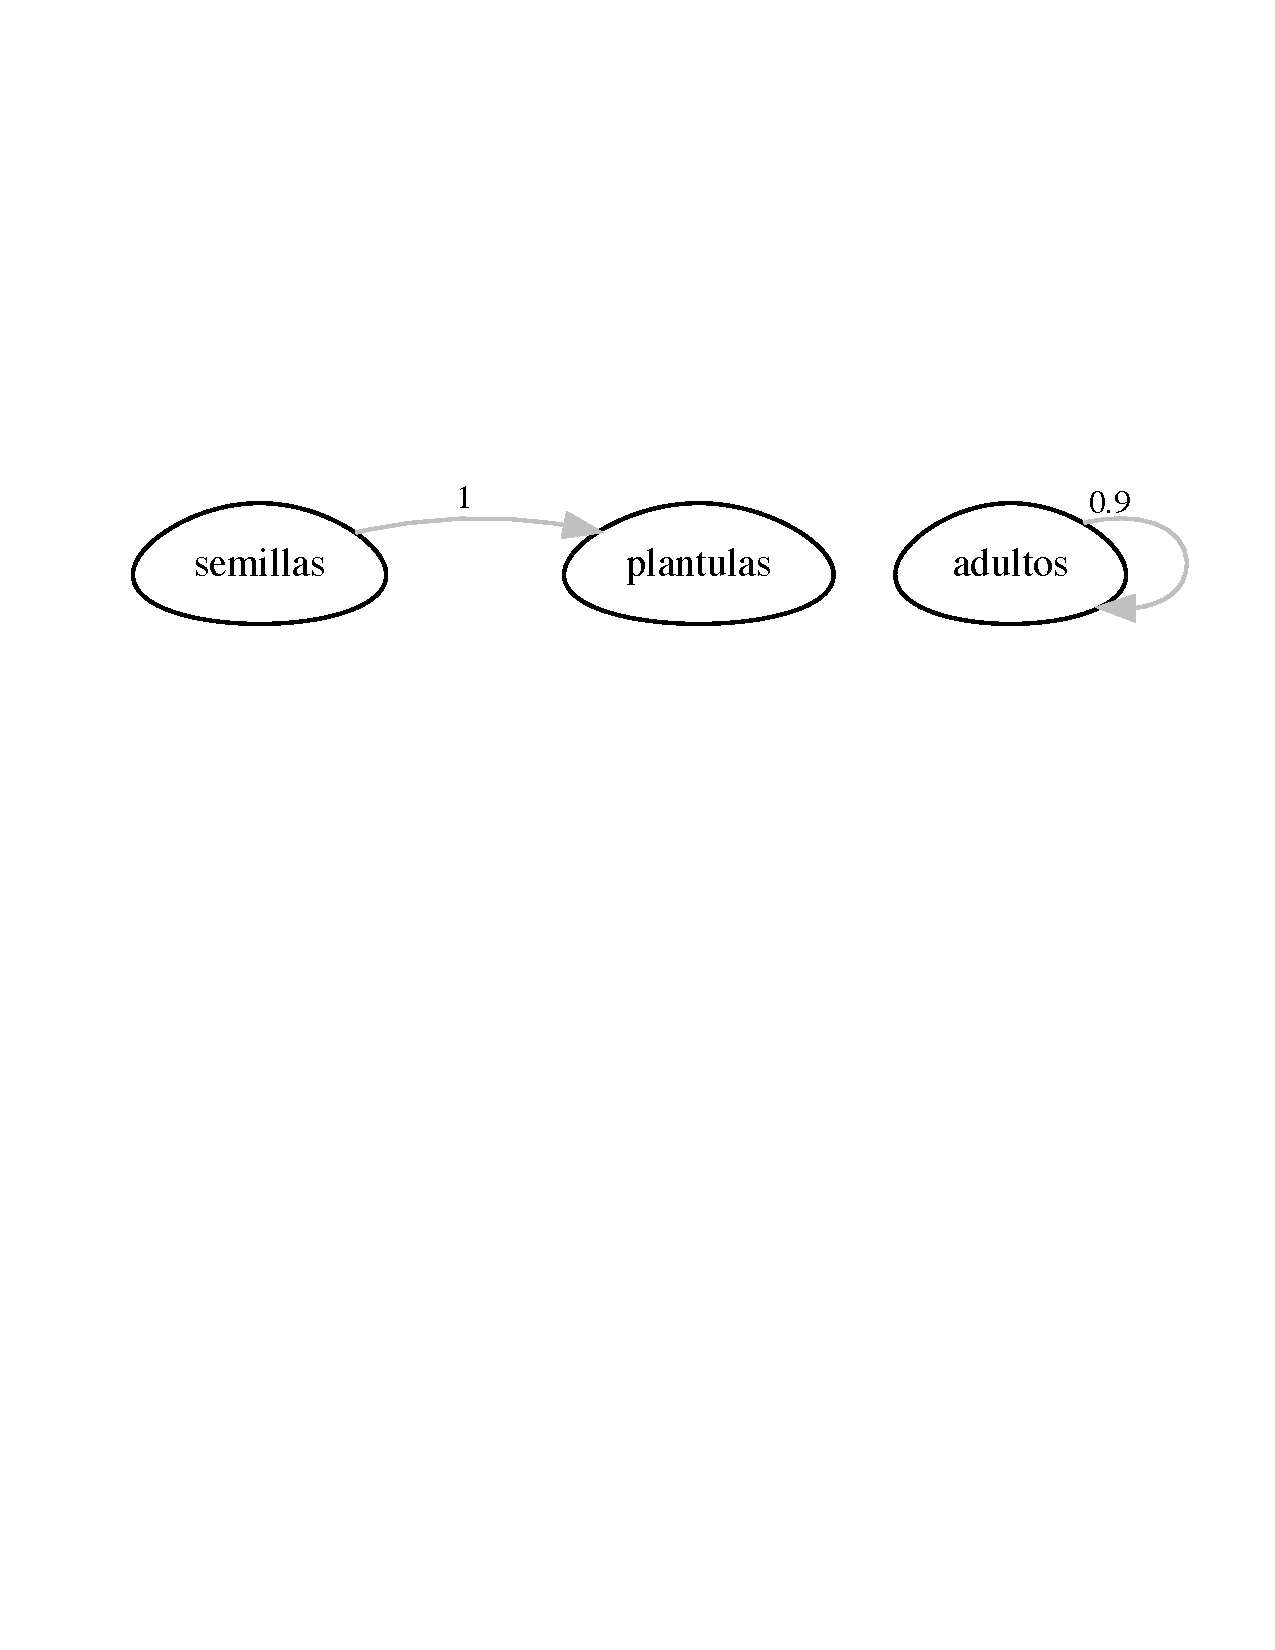
\includegraphics{108-Bayesian_PPM_files/figure-pdf/bayes2-1.pdf}

\subsection{Interpretaciones biológicamente irreales de los datos
existentes.}\label{interpretaciones-bioluxf3gicamente-irreales-de-los-datos-existentes.}

Al estudiar especies longevas como Sequoia sempervirens, es común
enfrentar interpretaciones erróneas derivadas de datos limitados o mal
contextualizados. Esta especie puede alcanzar tamaños extraordinarios
(diámetros a la altura del pecho, dbh, mayores a 3 metros) y tener una
longevidad estimada entre 1,200 y 2,200 años.

Supongamos que se realiza un muestreo de más de 1,000 individuos
grandes. Es posible que, en un intervalo de uno o incluso diez años, no
se observe la muerte de ningún individuo. A partir de estos datos, se
podría concluir erróneamente que la supervivencia anual es del 100\%.
Sin embargo, esta interpretación es biológicamente poco realista por
varias razones:

\begin{enumerate}
\def\labelenumi{\arabic{enumi}.}
\item
  \textbf{Tamaño de muestra insuficiente}: Si el muestreo se ampliara a
  10,000 o 100,000 individuos, probablemente se detectarían muertes,
  aunque fueran pocas. Esto sugiere que la mortalidad es baja, pero no
  nula.
\item
  \textbf{Relación entre tamaño y mortalidad}: En plantas, la
  probabilidad de morir suele disminuir con el tamaño del individuo. Los
  árboles más grandes tienen mayor resistencia a factores ambientales y
  biológicos, lo que reduce su tasa de mortalidad.
\item
  \textbf{Dependencia temporal de la mortalidad}: La muerte de
  individuos puede estar influenciada por eventos bióticos (plagas,
  enfermedades) o abióticos (sequías, incendios, tormentas) que varían
  entre años. En años extremos, la mortalidad puede aumentar
  significativamente.
\end{enumerate}

Por lo tanto, aunque los datos observados sugieren una supervivencia
perfecta, la probabilidad real de mortalidad es baja pero no cero. Este
tipo de sesgo en la interpretación puede ser corregido mediante enfoques
estadísticos más robustos, como el uso de modelos bayesianos que
incorporan incertidumbre y conocimiento previo sobre la biología de la
especie.

\begin{center}\rule{0.5\linewidth}{0.5pt}\end{center}

\section{El paquete ``raretrans''}\label{el-paquete-raretrans}

El siguiente sección usaremos el paquete ``raretrans'' que facilita los
estimados de las entradas en la matrices de transicione y fecundidades.
El manuscrito Tyre, Tremblay \& Perez (2024) contiene los datos
originales y el uso del paquete. Para tener acceso a los documentos
siguen el siguiente enlace
https://doi.org/10.1016/j.ecolmodel.2021.109526.

\textbf{Population projections from holey matrices: Using prior
information to estimate rare transition events}

Resumen

Las matrices de proyección poblacional (MPM) son una herramienta común
para predecir el comportamiento de la población a corto y largo plazo.
Sin embargo, cuando se utilizan para especies raras, amenazadas y en
peligro de extinción los datos disponibles suelen tener tamaños de
muestra reducido. En consecuencia, algunos eventos demográficos podrían
perderse en la modelización dando como resultado matrices con eventos
faltantes que reflejen trayectorias de ciclo de vida incompletas o
biológicamente poco realistas. Estas matrices con eventos faltantes
(ceros; e.g., sin observación de semillas que se transforman en
plántulas) a menudo se sustituyen utilizando información de la
literatura aunque información referente a otras poblaciones, otros
períodos de tiempo, otras especies usualmente se omite.

Una forma de abordar este problema es a través de métodos bayesianos
para el ajuste de los parámetros matriciales. Este marco estadístico nos
permite usar información previa para completar los valores faltantes
usando, por ejemplo, una distribución de Dirichlet para incluir
información sobre las transiciones de estado y una distribución Gamma
como previa para la fecundidad. Este método permite integrar información
conocida (\emph{a priori}) e incluir explícitamente el peso de la
información previa en las distribuciones posteriores. Además, al
establecer explícitamente las distribuciones previas, los resultados son
reproducibles y se pueden volver a evaluar con diferentes distribuciones
\emph{a priori} en el futuro. A continuación mostramos cómo el uso de
estos métodos en datos reales influye en la dispersión de los resultados
posteriores y origina matrices irreducibles y ergódicas, permitiendo
hacer inferencias biológicamente más realistas sobre las probabilidades
de transición y fertilidad.

\section{Instalación del paquete
raretrans}\label{instalaciuxf3n-del-paquete-raretrans}

Para instalar el paquete \texttt{raretrans}, es necesario habilitar el
acceso al código eliminando el símbolo \texttt{\#} que precede las
líneas del script de instalación. Esto permitirá ejecutar correctamente
las funciones del paquete.

Si tienes dificultades para instalar el paquete directamente desde R,
puedes acceder al repositorio oficial en GitHub y descargar las
funciones manualmente desde el siguiente enlace.

https://github.com/atyre2/raretrans/blob/master/raretrans.Rproj

Una vez descargado, puedes cargar las funciones en tu entorno de trabajo
en R utilizando \texttt{source()} o integrarlas en tu proyecto según sea
necesario.

\begin{Shaded}
\begin{Highlighting}[]
\NormalTok{devtools}\SpecialCharTok{::}\FunctionTok{install\_github}\NormalTok{(}\StringTok{"atyre2/raretrans"}\NormalTok{, }\AttributeTok{build =} \ConstantTok{TRUE}\NormalTok{, }\AttributeTok{build\_opts =} \FunctionTok{c}\NormalTok{(}\StringTok{"{-}{-}no{-}resave{-}data"}\NormalTok{, }\StringTok{"{-}{-}no{-}manual"}\NormalTok{)) }\CommentTok{\# instalar el paquete raretrans}

\FunctionTok{library}\NormalTok{(raretrans)}
\end{Highlighting}
\end{Shaded}

Ver el siguiente enlace para más información, la información que se
presenta a continuación es una traducción y ampliación de la información
del siguiente enlace. A continuación se muestra el uso del paquete
\texttt{raretrans} para estimar los parámetros en una población y en un
periodo de transición determinados.

\url{https://atyre2.github.io/raretrans/articles/onepopperiod.html}

A continuación se ejemplifica el uso del paquete \texttt{raretrans} para
estimar los parámetros en una población y en un periodo de transición
determinados.

\begin{Shaded}
\begin{Highlighting}[]
\CommentTok{\# Mi tema de formato de las gráficas de ggplot2 personal}
\NormalTok{rlt\_theme }\OtherTok{\textless{}{-}} \FunctionTok{theme}\NormalTok{(}\AttributeTok{axis.title.y =} \FunctionTok{element\_text}\NormalTok{(}\AttributeTok{colour=}\StringTok{"grey20"}\NormalTok{,}\AttributeTok{size=}\DecValTok{15}\NormalTok{,}\AttributeTok{face=}\StringTok{"bold"}\NormalTok{),}
        \AttributeTok{axis.text.x =} \FunctionTok{element\_text}\NormalTok{(}\AttributeTok{colour=}\StringTok{"grey20"}\NormalTok{,}\AttributeTok{size=}\DecValTok{15}\NormalTok{, }\AttributeTok{face=}\StringTok{"bold"}\NormalTok{),}
        \AttributeTok{axis.text.y =} \FunctionTok{element\_text}\NormalTok{(}\AttributeTok{colour=}\StringTok{"grey20"}\NormalTok{,}\AttributeTok{size=}\DecValTok{15}\NormalTok{,}\AttributeTok{face=}\StringTok{"bold"}\NormalTok{),  }
        \AttributeTok{axis.title.x =} \FunctionTok{element\_text}\NormalTok{(}\AttributeTok{colour=}\StringTok{"grey20"}\NormalTok{,}\AttributeTok{size=}\DecValTok{15}\NormalTok{,}\AttributeTok{face=}\StringTok{"bold"}\NormalTok{))}
\end{Highlighting}
\end{Shaded}

\section{Obtención de la matriz de
proyección}\label{obtenciuxf3n-de-la-matriz-de-proyecciuxf3n}

\texttt{raretrans} supone que la matriz de proyección es una lista con
dos componentes:

\begin{itemize}
\item
  \textbf{Matriz de transición}: Probabilidades de pasar de una etapa a
  otra (o permanecer en la misma).
\item
  \textbf{Matriz de fertilidad} Número de nuevos individuos producidos
  por cada etapa reproductiva.
\end{itemize}

Este es el formato de salida de \texttt{popbio::projection.matrix}. Si
tenemos transiciones individuales en nuestra base de datos (con clase
\texttt{data.frame()}), podemos usar
\texttt{raretrans::get\_state\_vector} para obtener el número inicial de
individuos por etapa.

Podemos utilizar la función \texttt{popbio::projection.matrix} para
obtener los datos necesarios. Hacemos una demostración con los datos de
transición y fertilidad de \emph{Lepanthes eltoroensis} \textbf{POPNUM
250} en el \textbf{periodo 5}. \emph{Lepanthes eltoroensis} es una
orquídea epífita, endémica de Puerto Rico y con una distribución
limitada a una pequeña región de la isla.

\begin{figure}[H]

{\centering 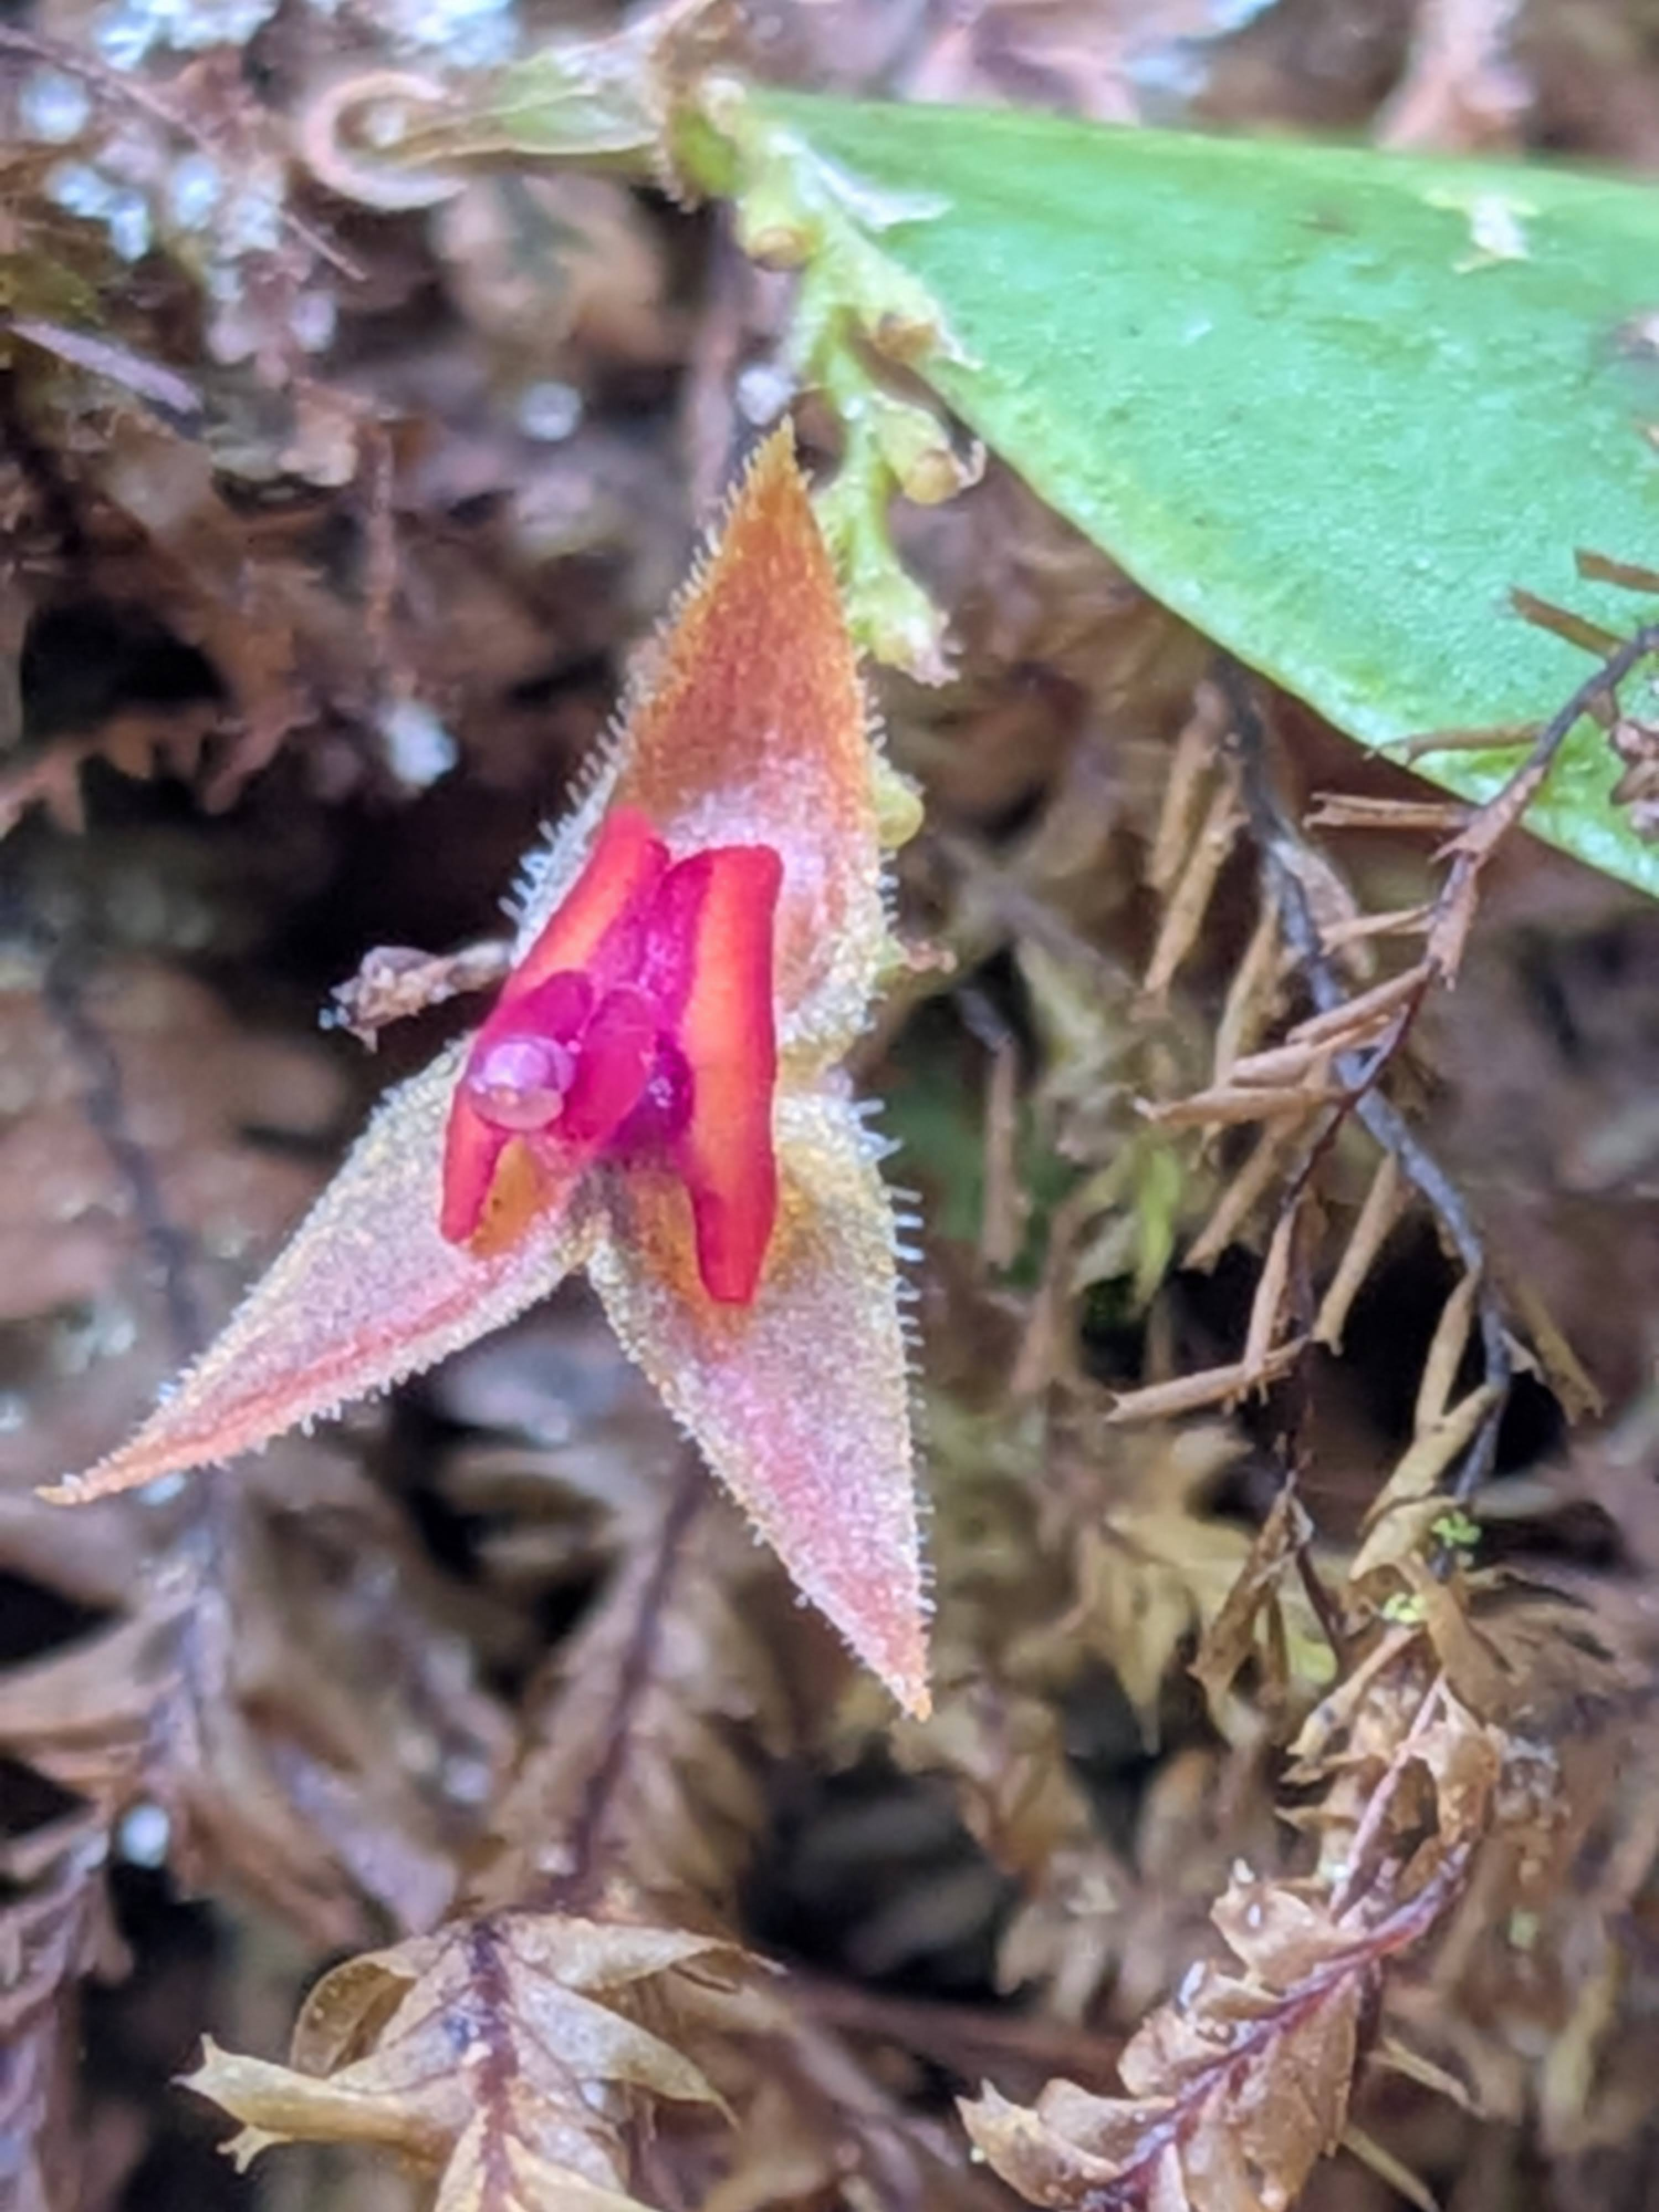
\includegraphics{Species/Lepanthes_eltoroensis_Edwin_Guevara.jpg}

}

\caption{\emph{Lepanthes eltoroensis}. Foto: Edwin Guevara}

\end{figure}%%
\begin{figure}[H]

{\centering 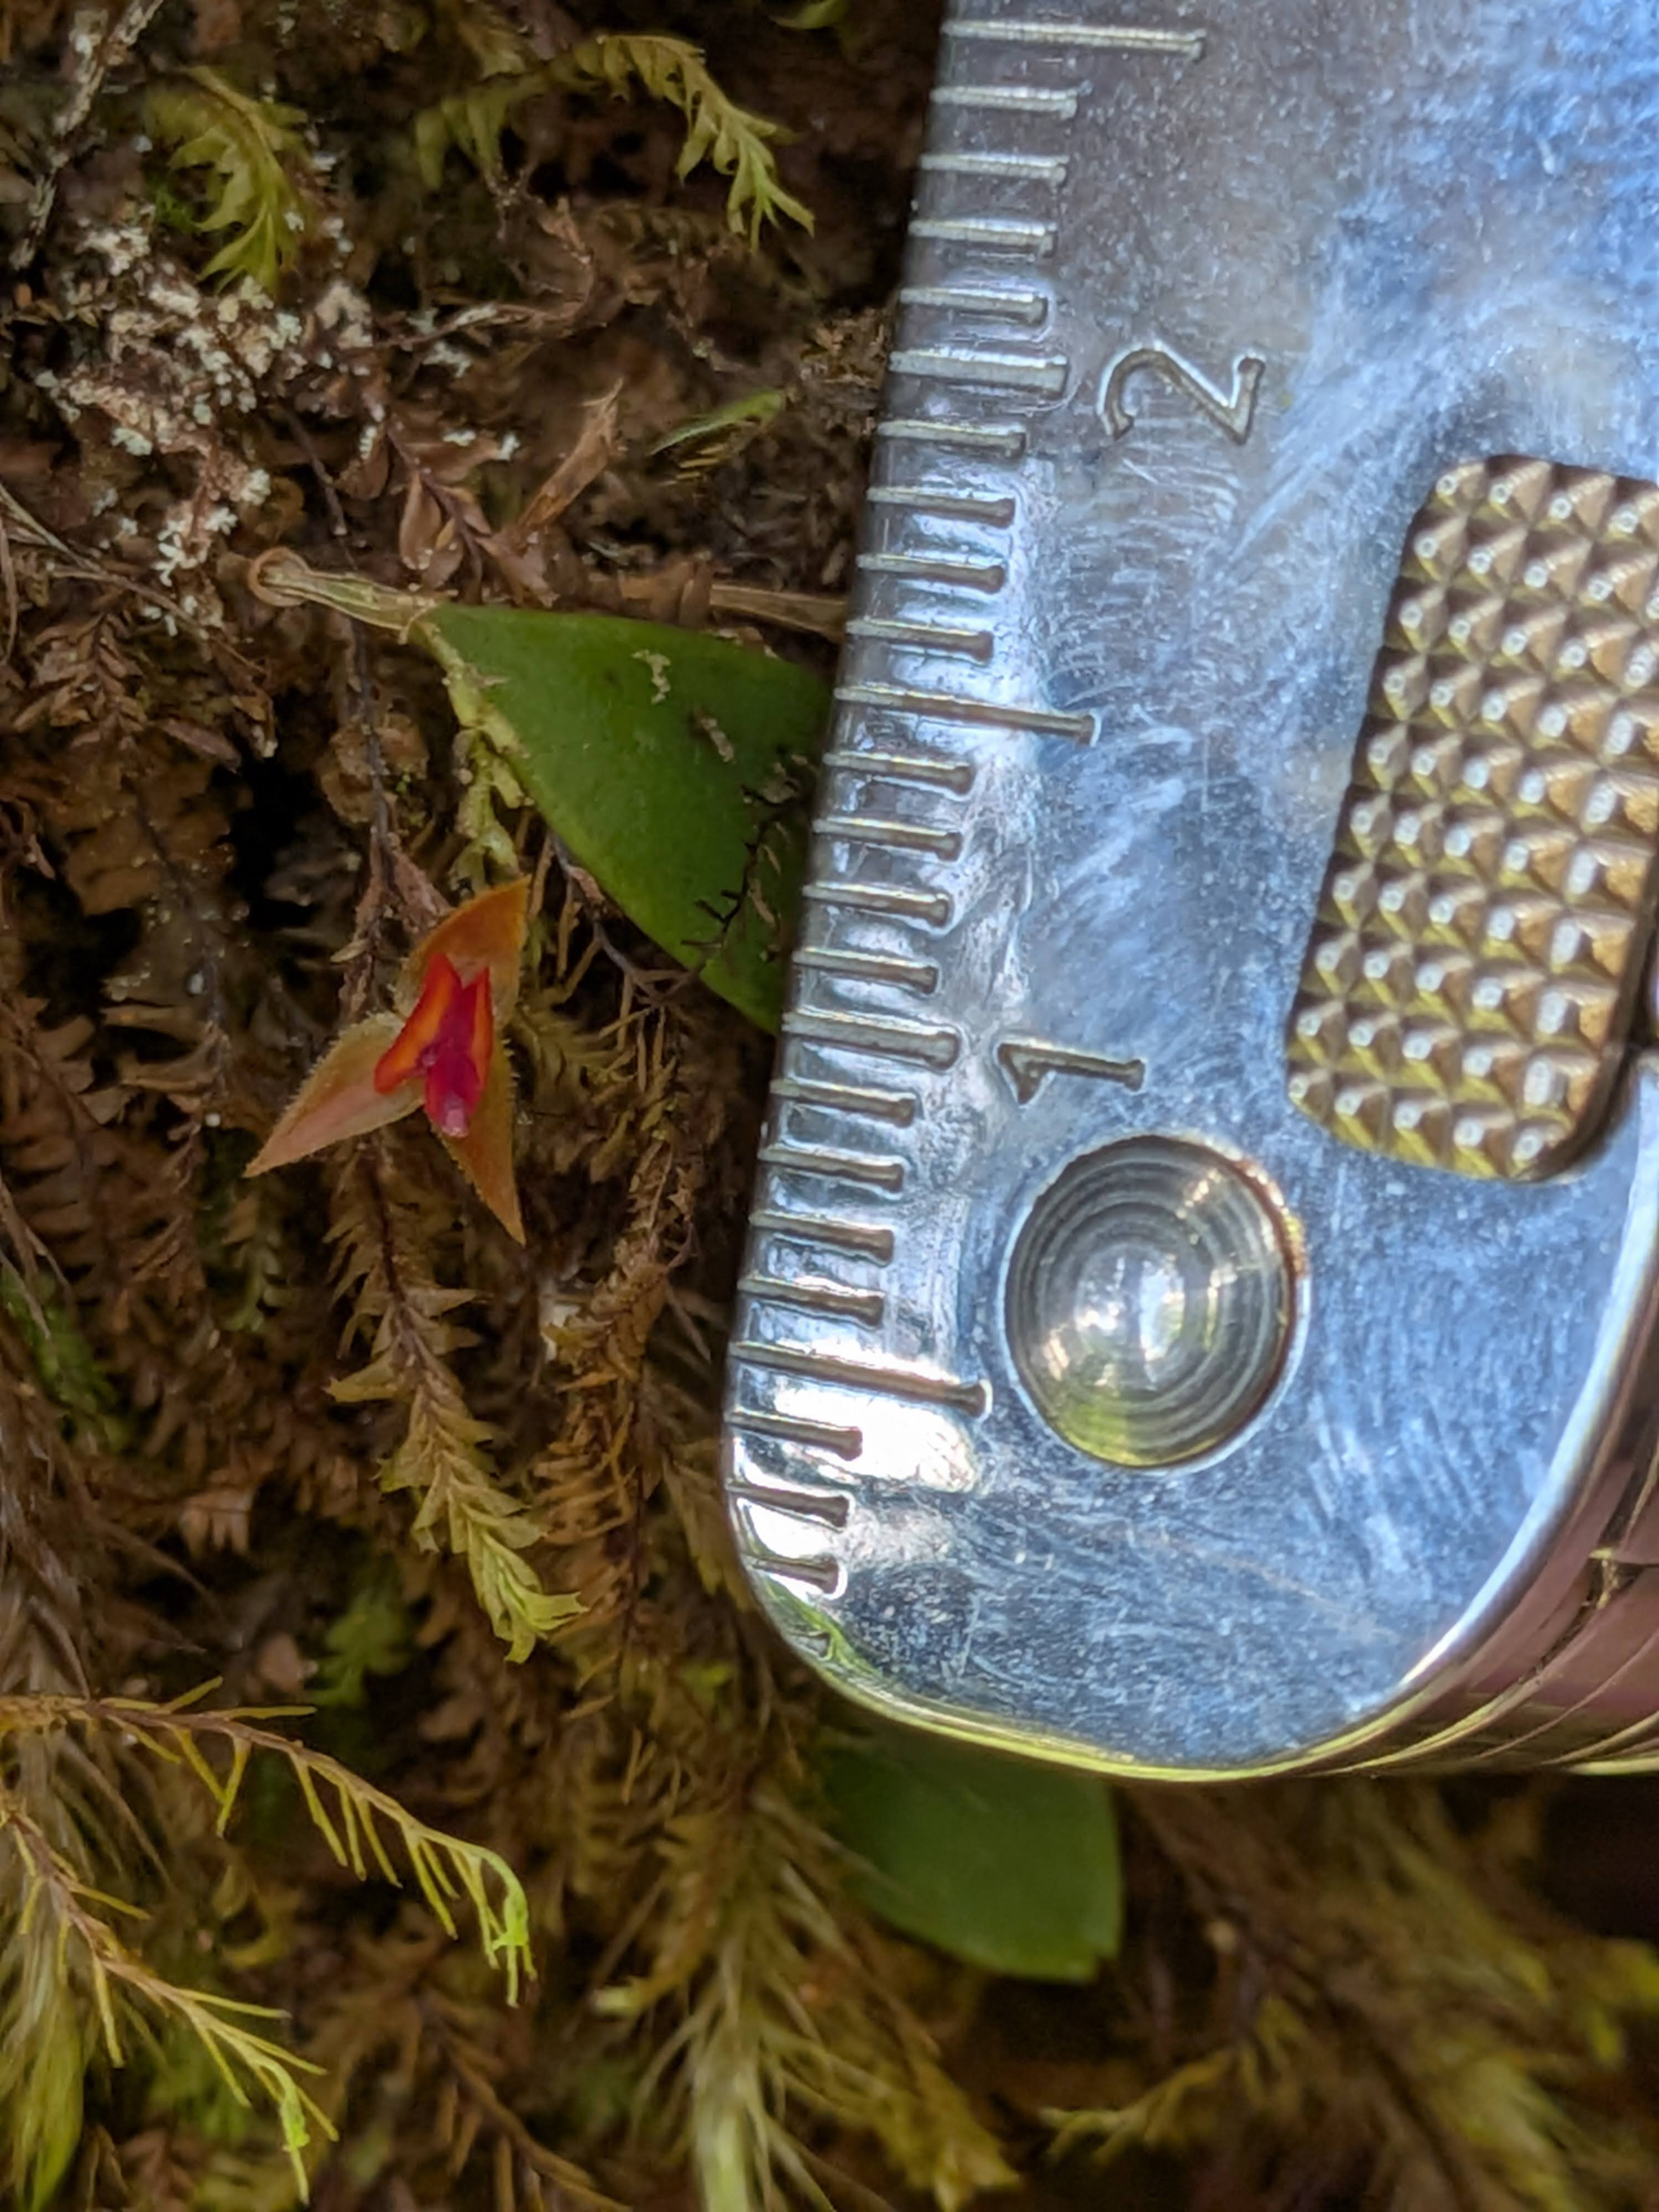
\includegraphics{Species/Lepanthes_eltoroensis_Phorophyte_Edwin_Guevara.jpg}

}

\caption{Lepanthes eltoroensis. Foto: Edwin Guevara}

\end{figure}%

\begin{center}\rule{0.5\linewidth}{0.5pt}\end{center}

\section{\texorpdfstring{Descargar los datos de la una población de
\emph{L. elto} del paquete
\textbf{raretrans}}{Descargar los datos de la una población de L. elto del paquete raretrans}}\label{descargar-los-datos-de-la-una-poblaciuxf3n-de-l.-elto-del-paquete-raretrans}

\begin{Shaded}
\begin{Highlighting}[]
\FunctionTok{data}\NormalTok{(}\StringTok{"L\_elto"}\NormalTok{) }\CommentTok{\# carga el conjunto de datos \textasciigrave{}L\_elto\textasciigrave{} en la memoria de la computadora (los datos están incluido en el paquete \textasciigrave{}raretrans\textasciigrave{})}
\FunctionTok{head}\NormalTok{(L\_elto) }
\end{Highlighting}
\end{Shaded}

\begin{verbatim}
# A tibble: 6 x 13
  POPNUM  year seedlings adults fertility IND_NUM stage next_stage first_year
   <dbl> <dbl>     <dbl>  <dbl>     <dbl>   <dbl> <chr> <chr>           <dbl>
1    209     1         1      6         0      67 j     j                   1
2    209     1         1      6         0      68 a     a                   1
3    209     1         1      6         0      69 a     a                   1
4    209     1         1      6         0      70 a     a                   1
5    209     1         1      6         0      71 j     a                   1
6    209     1         1      6         0      72 a     a                   1
# i 4 more variables: last_year <dbl>, recruited <lgl>, died <dbl>,
#   lifespan <int>
\end{verbatim}

\section{Organización de los datos en el
``data.frame''}\label{organizaciuxf3n-de-los-datos-en-el-data.frame}

Supongamos que tienes una base de datos llamada L\_elto con las
siguientes columnas:

\begin{itemize}
\tightlist
\item
  pop: identificador de la población
\item
  period: periodo de tiempo
\item
  stage: etapa actual del individuo
\item
  next\_stage: etapa siguiente
\item
  fertility: indicador de fertilidad
\end{itemize}

Seleccionamos la población POPNUM 250 y el periodo 5:

El primer paso es seleccionar los datos de la población y el periodo de
tiempo que queremos analizar. Posteriormente, cambiamos el nombre del
estado más pequeño a ``seedling''. Este paso no es estrictamente
necesario pero nos ayuda a entender más fácilmente la nomenclatura.

La base de datos \texttt{L\_elto} está compuesta por datos individuales
del estado actual (\texttt{stage}, periodo \textbf{t}), del estado
siguiente (\texttt{next\_stage}, periodo \textbf{t+1}) y de la
fertilidad. Tenga en cuenta que aquí ``p'' significa ``plántula'' por la
traducción al español. En la siguiente caja de código las primeras
líneas seleccionan la población de interés y el periodo de tiempo sobre
el que queremos trabajar y cambian el nombre de la etapa del ciclo vital
de ``p'' a ``s''.

\begin{Shaded}
\begin{Highlighting}[]
\NormalTok{onepop }\OtherTok{\textless{}{-}}\NormalTok{ L\_elto }\SpecialCharTok{\%\textgreater{}\%}

  \FunctionTok{filter}\NormalTok{(POPNUM }\SpecialCharTok{==} \DecValTok{250}\NormalTok{, year }\SpecialCharTok{==} \DecValTok{5}\NormalTok{) }\SpecialCharTok{\%\textgreater{}\%} \CommentTok{\# Filtrar la población \# 250, el periodo (año=year) 5}

  \FunctionTok{mutate}\NormalTok{(}
    \AttributeTok{stage =} \FunctionTok{case\_when}\NormalTok{(stage }\SpecialCharTok{==} \StringTok{"p"} \SpecialCharTok{\textasciitilde{}} \StringTok{"s"}\NormalTok{, }\ConstantTok{TRUE} \SpecialCharTok{\textasciitilde{}}\NormalTok{ stage),}
    \AttributeTok{next\_stage =} \FunctionTok{case\_when}\NormalTok{(next\_stage }\SpecialCharTok{==} \StringTok{"p"} \SpecialCharTok{\textasciitilde{}} \StringTok{"s"}\NormalTok{, }\ConstantTok{TRUE} \SpecialCharTok{\textasciitilde{}}\NormalTok{ next\_stage)}
\NormalTok{  ) }\CommentTok{\# redefine "p" por plantula a "s" para seedling}
\end{Highlighting}
\end{Shaded}

En el siguiente código usamos la función
\texttt{popbio::projection.matrix()} para crear la matriz de proyección
poblacional. Tenemos ahora nuestra matriz de transición y fecundidad
basado en los datos de la población \#250 del periodo 5. La función
\texttt{projection.matrix()} requiere que se especifiquen los nombres de
las etapas y los estados siguientes, así como el nombre de la columna de
fertilidad. En este caso, las etapas son ``s'' (plántula), ``j''
(juvenil) y ``a'' (adulto), y el estado siguiente es
\texttt{next\_stage}. La columna de fertilidad se llama
\texttt{fertility}. El argumento \texttt{sort} especifica el orden en
que queremos que aparezcan las etapas en la matriz.

Solamente los adultos pueden producir plántulas, por lo que la matriz de
fertilidad tiene un valor de fertilidad solamente en la posición (1,3),
(plántula, adulto). La función \texttt{projection.matrix()} devuelve una
lista con dos matrices: una de transición y otra de fertilidad. La
matriz de transición es una matriz cuadrada que muestra las
probabilidades de transición entre las etapas, mientras que la matriz de
fertilidad es una matriz que muestra la fecundidad por etapa.

A partir de este punto los análisis se llevan a cabo considerando
\textbf{s} (plántula), \textbf{j} (juvenil) y \textbf{a} (adulto), y las
dos matrices: \textbf{T} (transición de estadios) y \textbf{F}
(fertilidad). La tasa de crecimiento asintótica de la población
observada es \(\lambda\). Las transiciones raras que faltan en nuestra
primera matriz de transición `TF\$T', pero que sabemos que ocurren, son
la transición de plántula (\emph{s}) a adulto (\emph{a}) y la transición
de \emph{j} a \emph{s}.

\begin{Shaded}
\begin{Highlighting}[]
\CommentTok{\# popbio::projection.matrix no funciona con el formato *tibbles*, por consecuencia se convierte en data.frame}

\FunctionTok{head}\NormalTok{(onepop) }\CommentTok{\# Ahora tenemos solamente datos de la población \#250 del periodo 5}
\end{Highlighting}
\end{Shaded}

\begin{verbatim}
# A tibble: 6 x 13
  POPNUM  year seedlings adults fertility IND_NUM stage next_stage first_year
   <dbl> <dbl>     <dbl>  <dbl>     <dbl>   <dbl> <chr> <chr>           <dbl>
1    250     5         8     34     0         167 j     a                   1
2    250     5         8     34     0         168 j     a                   1
3    250     5         8     34     0         169 j     a                   1
4    250     5         8     34     0.118     170 a     a                   1
5    250     5         8     34     0         172 j     j                   1
6    250     5         8     34     0         173 j     a                   1
# i 4 more variables: last_year <dbl>, recruited <lgl>, died <dbl>,
#   lifespan <int>
\end{verbatim}

\begin{Shaded}
\begin{Highlighting}[]
\CommentTok{\# Crear TF = TRUE, añadir para formatear correctamente.}
\NormalTok{TF }\OtherTok{\textless{}{-}}\NormalTok{ popbio}\SpecialCharTok{::}\FunctionTok{projection.matrix}\NormalTok{(}
  \FunctionTok{as.data.frame}\NormalTok{(onepop),}
  \AttributeTok{stage =}\NormalTok{ stage,}
  \AttributeTok{fate =}\NormalTok{ next\_stage,}
  \AttributeTok{fertility =} \StringTok{"fertility"}\NormalTok{,}
  \AttributeTok{sort =} \FunctionTok{c}\NormalTok{(}\StringTok{"s"}\NormalTok{, }\StringTok{"j"}\NormalTok{, }\StringTok{"a"}\NormalTok{),}
  \AttributeTok{TF =} \ConstantTok{TRUE}
\NormalTok{)}
\NormalTok{TF }\CommentTok{\# Este es la estructura de etapas de vida para esa población.  Nota que tenemos dos matrices, una de transiciones **T** y otra de fertilidad **F**.}
\end{Highlighting}
\end{Shaded}

\begin{verbatim}
$T
   
             s          j          a
  s 0.09090909 0.00000000 0.00000000
  j 0.63636364 0.57446809 0.00000000
  a 0.00000000 0.29787234 0.85294118

$F
   
            s         j         a
  s 0.0000000 0.0000000 0.1176471
  j 0.0000000 0.0000000 0.0000000
  a 0.0000000 0.0000000 0.0000000
\end{verbatim}

\begin{center}\rule{0.5\linewidth}{0.5pt}\end{center}

\section{Obtener el número inicial de individuos por
etapa}\label{obtener-el-nuxfamero-inicial-de-individuos-por-etapa}

Dado que nuestros conteos (número de individuos), \(N\) y el tamaño de
\emph{muestra equivalente} \emph{a priori} se expresan como múltiplos
del número de individuos observados, necesitamos obtener el número de
individuos en cada etapa (\(N\)) en el primer periodo de tiempo. Para
esto utilizamos la función \texttt{raretrans::get\_state\_vector()}. Se
observa que la cantidad de individuos iniciales por etapa es el número
de individuos en el primer muestreo es muy limitada, con 11 plántulas,
47 juveniles y 34 adultos, para esta población en este periodo de
muestreo.

\begin{Shaded}
\begin{Highlighting}[]
\NormalTok{N }\OtherTok{\textless{}{-}} \FunctionTok{get\_state\_vector}\NormalTok{(onepop, }\AttributeTok{stage =}\NormalTok{ stage, }\AttributeTok{sort =} \FunctionTok{c}\NormalTok{(}\StringTok{"s"}\NormalTok{, }\StringTok{"j"}\NormalTok{, }\StringTok{"a"}\NormalTok{))}
\NormalTok{N }\CommentTok{\# Un vector \# de individuos iniciales para cada etapa, nota que la cantidad por etapa, "stage", son los individuos en el primer muestreo}
\end{Highlighting}
\end{Shaded}

\begin{verbatim}
[1] 11 47 34
\end{verbatim}

\section{Método alterno para calcular transiciones, fertilidades y el
número de individuos por
etapas.}\label{muxe9todo-alterno-para-calcular-transiciones-fertilidades-y-el-nuxfamero-de-individuos-por-etapas.}

La lista de matrices y el vector de conteos de individuos no tienen por
qué proceder de un ``data frame'' como hemos hecho anteriormente.
Mientras tengan el formato esperado, pueden crearse a mano. Usemos la
población 231 en el periodo 2 como ejemplo para dividir la matriz
poblacional en la submatrices de transición \textbf{T} y de fertilidad
\textbf{F}. En el siguiente código, \emph{m} denota mortalidad, es
decir, plantas que están muertas. Note que aquí las transiciones están
estimadas con un tamaño de muestra todavía más pequeño, solamente 2
plántulas, 6 juveniles y 16 adultos. Ninguna de las 2 plántulas pasaron
a la etapa de juveniles. En consecuencia esta transición es de cero.
Además, una de estas plántulas murió, por lo que la supervivencia es del
50\%. Sin embargo, si hubieran muerto las dos plántulas la mortalidad
sería del 100\% y si hubieran sobrevivido las dos plántulas sería del
100\% ¡No hay valores intermedios!

La matriz de transición y la matriz de fertilidad y el vector de tamaño
poblacional para la población 231, periodo 2 son:

\begin{Shaded}
\begin{Highlighting}[]
\NormalTok{TF2}
\end{Highlighting}
\end{Shaded}

\begin{verbatim}
$Tmat
    stage
fate         p         j         a
   p 0.5000000 0.0000000 0.0000000
   j 0.0000000 0.8333333 0.0000000
   a 0.0000000 0.1666667 0.8750000

$Fmat
     [,1] [,2]  [,3]
[1,]    0    0 0.125
[2,]    0    0 0.000
[3,]    0    0 0.000
\end{verbatim}

\begin{Shaded}
\begin{Highlighting}[]
\NormalTok{N2}
\end{Highlighting}
\end{Shaded}

\begin{verbatim}
 p  j  a 
 2  6 16 
\end{verbatim}

\begin{center}\rule{0.5\linewidth}{0.5pt}\end{center}

\subsection{¿Cómo se ve el ciclo de vida de la población en ese
periodo?}\label{cuxf3mo-se-ve-el-ciclo-de-vida-de-la-poblaciuxf3n-en-ese-periodo}

A la matriz mostrada le falta la transición de plántula a juvenil.
Ademas dado que ninguno de los 6 juveniles murió hay una sobrestimación
de su supervivencia. La tasa de crecimiento asintótica de la población
observada es \(\lambda\). La matriz no es ergódica (no se puede llegar a
cualquier otro estado desde uno o más estados), y es reducible, lo que
significa que una o más columnas y filas se pueden descartar y tienen
las mismas propiedades en términos de sus eigenvalores y eigenvectores.

Lo que vimos anteriormente fueron algunos de los problemas reales que
encontramos cuando usamos datos de campo y hay tamaños de muestra
pequeños o transiciones raras. A continuación veremos cómo resolverlos.

\begin{Shaded}
\begin{Highlighting}[]
\NormalTok{stages2 }\OtherTok{\textless{}{-}} \FunctionTok{c}\NormalTok{(}\StringTok{"plantulas"}\NormalTok{, }\StringTok{"juveniles"}\NormalTok{, }\StringTok{"adultos"}\NormalTok{)}
\NormalTok{title }\OtherTok{\textless{}{-}} \ConstantTok{NULL}
\FunctionTok{plot\_life\_cycle}\NormalTok{(Tmat, }\AttributeTok{stages =}\NormalTok{ stages2)}
\end{Highlighting}
\end{Shaded}

\begin{verbatim}
file:////private/var/folders/3k/1ft37x9130vdbz21tw1497x40000gn/T/RtmpV3jON5/file1035132ba74f4/widget103516f545930.html screenshot completed
\end{verbatim}

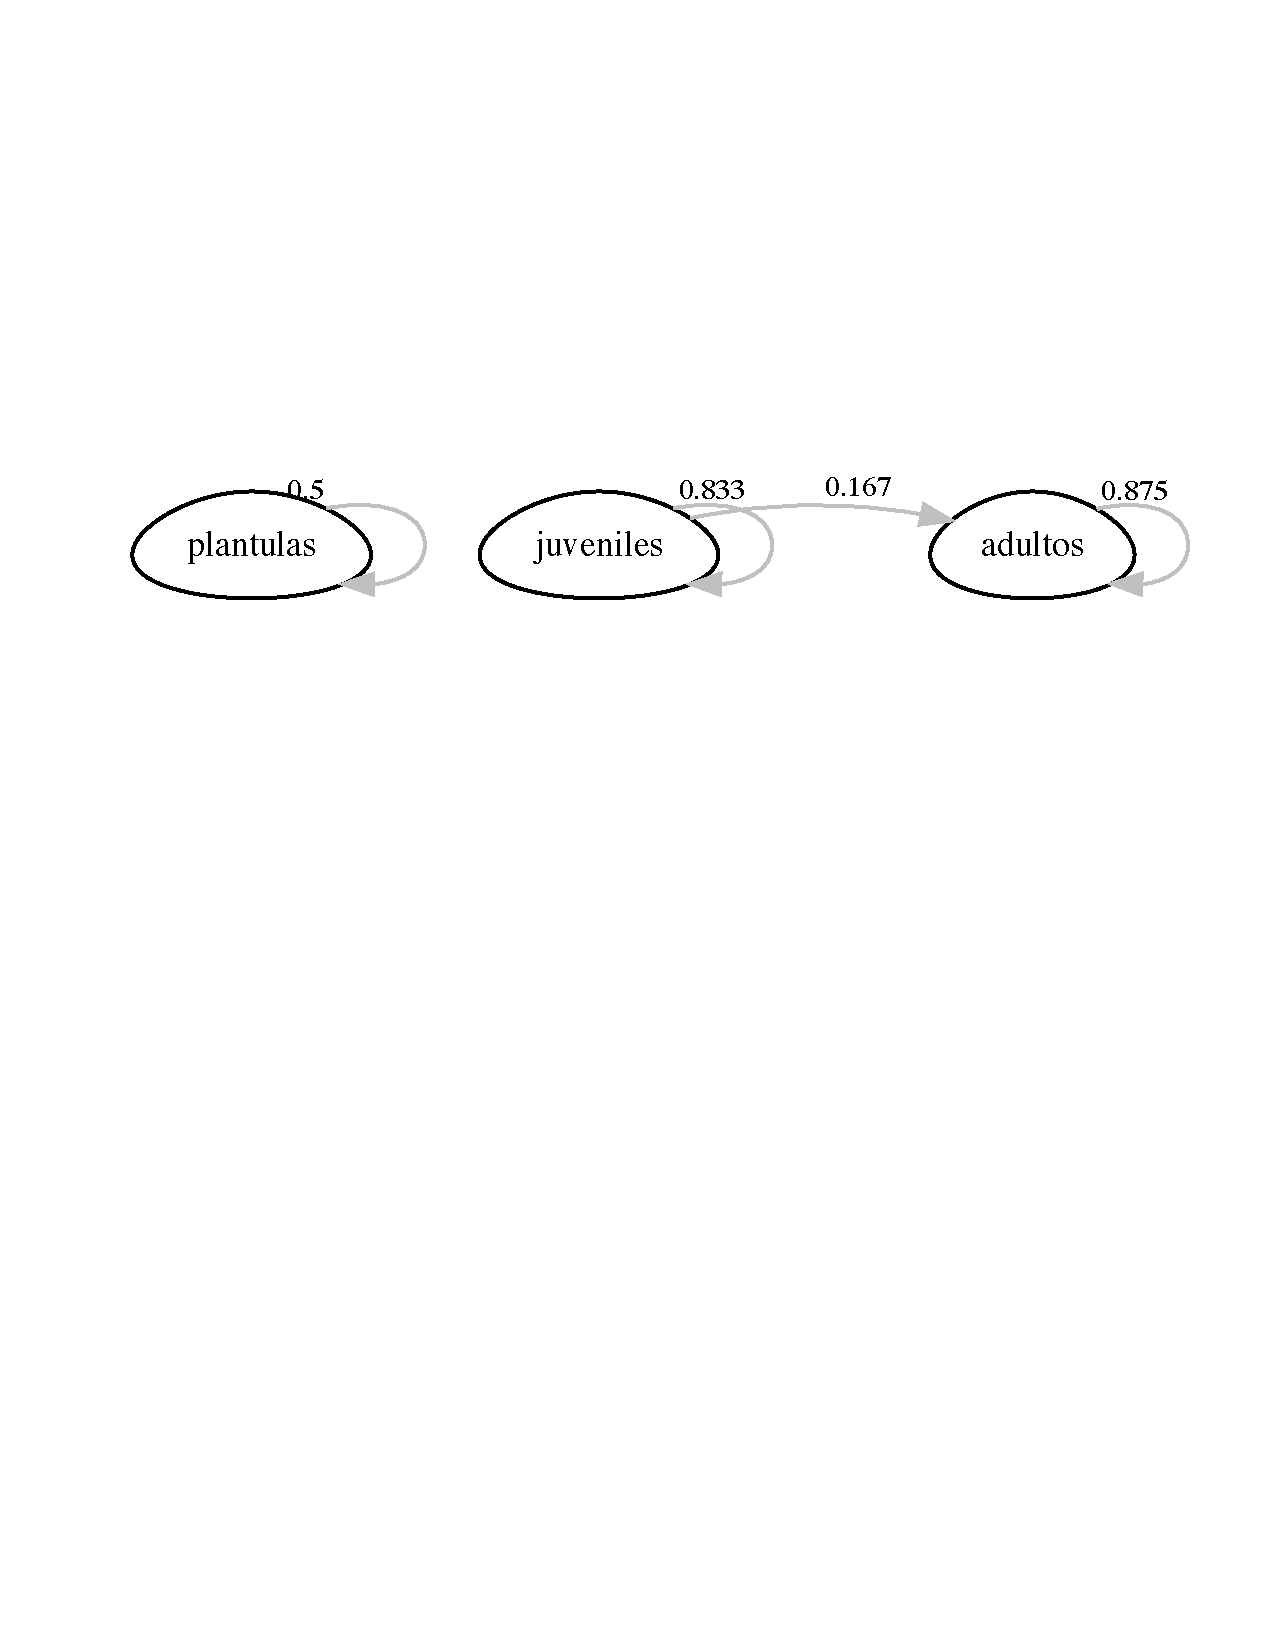
\includegraphics{108-Bayesian_PPM_files/figure-pdf/bayes11-1.pdf}

\begin{center}\rule{0.5\linewidth}{0.5pt}\end{center}

\subsection{Incorporar previas
informativas}\label{incorporar-previas-informativas}

Para evitar que el modelo genere transiciones imposibles entre etapas
del ciclo de vida, se pueden incorporar previas informativas. Estas
previas se basan en el conocimiento experto sobre la especie, en este
caso proporcionado por un especialista en orquídeas epífitas del género
Lepanthes (RLT). La información debe tener el mismo formato que la
matriz de transición, es decir:

\begin{itemize}
\tightlist
\item
  Una matriz con una fila más que columnas.
\item
  La última fila representa los individuos que mueren en cada etapa.
\end{itemize}

Es importante que estos valores se definan antes de recolectar los datos
de campo, para evitar que el análisis se vea influenciado o sesgado por
los datos observados.

\begin{Shaded}
\begin{Highlighting}[]
\NormalTok{RLT\_Tprior }\OtherTok{\textless{}{-}} \FunctionTok{matrix}\NormalTok{(}\FunctionTok{c}\NormalTok{(}\FloatTok{0.25}\NormalTok{, }\FloatTok{0.025}\NormalTok{, }\FloatTok{0.0}\NormalTok{,}
                       \FloatTok{0.05}\NormalTok{, }\FloatTok{0.9}\NormalTok{,   }\FloatTok{0.025}\NormalTok{,}
                       \FloatTok{0.01}\NormalTok{, }\FloatTok{0.025}\NormalTok{, }\FloatTok{0.95}\NormalTok{,}
                       \FloatTok{0.69}\NormalTok{, }\FloatTok{0.05}\NormalTok{,  }\FloatTok{0.025}\NormalTok{), }
                       \AttributeTok{byrow =} \ConstantTok{TRUE}\NormalTok{, }\AttributeTok{nrow =} \DecValTok{4}\NormalTok{, }\AttributeTok{ncol =} \DecValTok{3}\NormalTok{)}
\end{Highlighting}
\end{Shaded}

Note que la matriz tiene la 1ª fila, 3ª columna es 0,0, porque esta
transición es imposible. Las previas se construyen de manera que las
columnas sumen 1, lo que crea mayor flexibilidad para la ponderación de
los valores \emph{a priori}. Por defecto, la suma es 1, interpretado
como un \emph{tamaño de muestra a priori} de 1.

A hora usando la función de \textbf{fill\_transitions} donde se agregan
los valores del campo \textbf{TF}, el tamaño de muestra en el tiempo
inicial \textbf{N}, la matriz de valores con \emph{priors} informativos,
y se calcula la matriz de transición \emph{a posteriori}. Compare
\textbf{TF} con esta matriz para ver los cambios.

\begin{Shaded}
\begin{Highlighting}[]
\FunctionTok{fill\_transitions}\NormalTok{(TF, N, }\AttributeTok{P =}\NormalTok{ RLT\_Tprior)}
\end{Highlighting}
\end{Shaded}

\begin{verbatim}
             [,1]         [,2]         [,3]
[1,] 0.1041666667 0.0005208333 0.0000000000
[2,] 0.5875000000 0.5812500000 0.0007142857
[3,] 0.0008333333 0.2921875000 0.8557142857
\end{verbatim}

\begin{center}\rule{0.5\linewidth}{0.5pt}\end{center}

\subsection{\texorpdfstring{Modificar el peso de los valores \emph{a
priori}}{Modificar el peso de los valores a priori}}\label{modificar-el-peso-de-los-valores-a-priori}

Cuando usamos previas informativas en el modelo, podemos ajustar su peso
modificando el tamaño de muestra a priori para cada etapa del ciclo de
vida.

\subsection{¿Por qué ajustar el peso?}\label{por-quuxe9-ajustar-el-peso}

\begin{itemize}
\tightlist
\item
  Si tenemos alta confianza en los valores a priori (por ejemplo, por
  experiencia o estudios previos), podemos asignarles un peso mayor.
\item
  Si tenemos poca confianza, es mejor asignarles un peso pequeño,
  permitiendo que los datos de campo tengan mayor influencia en los
  resultados.
\end{itemize}

\subsubsection{¿Cómo se interpreta el
peso?}\label{cuxf3mo-se-interpreta-el-peso}

El peso se especifica como el tamaño de muestra a priori. Por defecto,
cada columna de la matriz de previas suma 1, lo que equivale a un tamaño
de muestra a priori de 1. Puedes modificar esta suma para reflejar mayor
o menor certeza en los valores propuestos.

\begin{Shaded}
\begin{Highlighting}[]
\FunctionTok{fill\_transitions}\NormalTok{(TF, N, }\AttributeTok{P =}\NormalTok{ RLT\_Tprior, }\AttributeTok{priorweight =} \FloatTok{0.5}\NormalTok{)}
\end{Highlighting}
\end{Shaded}

\begin{verbatim}
            [,1]        [,2]        [,3]
[1,] 0.143939394 0.008333333 0.000000000
[2,] 0.440909091 0.682978723 0.008333333
[3,] 0.003333333 0.206914894 0.885294118
\end{verbatim}

En este caso, el \texttt{priorweight} se pondera con la mitad del número
de transiciones observadas. Por ejemplo: Si se observaron solo 2
transiciones, entonces priorweight = 1, lo que equivale a un tamaño de
muestra a priori de 1. Si se observaran más transiciones, por ejemplo
20, entonces priorweight = 10, lo que permite que los datos observados
tengan mayor influencia en el resultado final.

\textbf{Recomendación} Siempre se debe asignar a las previas un peso
menor (preferiblemente mucho menor) que el tamaño de muestra observado.
Esto garantiza que los datos reales del campo tengan mayor peso en el
análisis y evita que el conocimiento previo domine injustamente los
resultados.

\textbf{Resultado}

La nueva matriz de transición:

\begin{itemize}
\tightlist
\item
  Es ergódica (todas las etapas están conectadas directa o
  indirectamente).
\item
  Es reducible, lo que significa que algunas etapas pueden no ser
  alcanzables desde otras, dependiendo del ciclo de vida.
\item
  Presenta tasas de mortandad y transición más realistas, gracias a la
  incorporación del conocimiento experto.
\end{itemize}

\begin{center}\rule{0.5\linewidth}{0.5pt}\end{center}

\section{Intervalos de credibilidad para las
transiciones}\label{intervalos-de-credibilidad-para-las-transiciones}

Una vez ajustada la matriz de transición con los datos observados y las
previas informativas, podemos calcular los intervalos de credibilidad
(ICr) para cada entrada de la matriz.

\textbf{¿Cómo se calculan?} Cada elemento de la matriz de transición
ajustada sigue una distribución beta, ya que proviene de una
distribución posterior marginal de una multinomial. Esto permite
calcular intervalos de credibilidad para las tasas de transición.

Para obtener estos valores, se puede usar el tipo de retorno TN, que
proporciona:

\begin{itemize}
\tightlist
\item
  La estimación puntual.
\item
  El límite inferior del intervalo de credibilidad al 95\%.
\item
  El límite superior del intervalo de credibilidad al 95\%.
\end{itemize}

\subsection{Ejemplo: etapa de
plántula}\label{ejemplo-etapa-de-pluxe1ntula}

Supongamos que estamos analizando las transiciones desde la etapa de
plántula (s). Si el número de transiciones observadas es 2, y el peso de
las previas es 1, el tamaño de muestra efectivo es 3. Esto genera un
intervalo de credibilidad más amplio, reflejando la alta incertidumbre
en la estimación. Por ejemplo:

\begin{itemize}
\tightlist
\item
  La tasa de mortandad puntual es 0.31.
\item
  El intervalo de credibilidad al 95\% va de 0.096 a 0.585.
\end{itemize}

Este rango amplio indica que el mejor estimado es muy incierto, lo cual
es típico cuando se trabaja con tamaños de muestra pequeños.

\subsection{Interpretación}\label{interpretaciuxf3n}

Un intervalo de credibilidad amplio significa que hay mucha
incertidumbre en la estimación del parámetro. Esto resalta la
importancia de contar con:

\begin{itemize}
\tightlist
\item
  Más datos de campo.
\item
  Previas bien fundamentadas.
\item
  Un análisis cuidadoso del tamaño de muestra efectivo.
\end{itemize}

\begin{Shaded}
\begin{Highlighting}[]
\NormalTok{TN }\OtherTok{\textless{}{-}} \FunctionTok{fill\_transitions}\NormalTok{(}
\NormalTok{  TF,}
\NormalTok{  N,}
  \AttributeTok{P =}\NormalTok{ RLT\_Tprior,}
  \AttributeTok{priorweight =} \FloatTok{0.1}\NormalTok{,}
  \AttributeTok{returnType =} \StringTok{"TN"}
\NormalTok{)}
\NormalTok{a }\OtherTok{\textless{}{-}}\NormalTok{ TN[, }\DecValTok{1}\NormalTok{] }\CommentTok{\# cambie 1 a 2, 3 etc para obtener la distribución beta marginal de cada columna (etapa de vida).}
\NormalTok{b }\OtherTok{\textless{}{-}} \FunctionTok{sum}\NormalTok{(TN[, }\DecValTok{1}\NormalTok{]) }\SpecialCharTok{{-}}\NormalTok{ TN[, }\DecValTok{1}\NormalTok{] }\CommentTok{\# cambie 1 a 2, 3 etc para obtener la distribución beta marginal de cada columna.}
\NormalTok{p }\OtherTok{\textless{}{-}}\NormalTok{ a }\SpecialCharTok{/}\NormalTok{ (a }\SpecialCharTok{+}\NormalTok{ b)}
\NormalTok{lcl }\OtherTok{\textless{}{-}} \FunctionTok{qbeta}\NormalTok{(}\FloatTok{0.025}\NormalTok{, a, b) }\CommentTok{\# el valor 0.025 de la distribución beta}
\NormalTok{ucl }\OtherTok{\textless{}{-}} \FunctionTok{qbeta}\NormalTok{(}\FloatTok{0.975}\NormalTok{, a, b) }\CommentTok{\# el valor 0.975 de la distribución beta}
\NormalTok{knitr}\SpecialCharTok{::}\FunctionTok{kable}\NormalTok{(}\FunctionTok{sprintf}\NormalTok{(}\StringTok{"\%.4f (\%.4f, \%.4f)"}\NormalTok{, p, lcl, ucl)) }\CommentTok{\# Crear una tabla con los resultados con 4 cifras decimales (note la ultima fila son los fallecidos)}
\end{Highlighting}
\end{Shaded}

\begin{longtable}[]{@{}l@{}}
\toprule\noalign{}
x \\
\midrule\noalign{}
\endhead
\bottomrule\noalign{}
\endlastfoot
0.1054 (0.0058, 0.3212) \\
0.5831 (0.3087, 0.8315) \\
0.0009 (0.0000, 0.0052) \\
0.3107 (0.0956, 0.5846) \\
\end{longtable}

Una de la gran ventaja de usar el paquete \texttt{raretrans} es que
podemos calcular los intervalos de credibilidad de las tasas de
transición y fertilidad de manera rápida y sencilla. Ademas que los
intervalos de credibilidad están limitado a los valores entre 0 y 1, lo
que es importante para las tasas de transición y fertilidad. Esto es
especialmente útil cuando se trabaja con datos de campo donde el tamaño
de muestra es pequeño y las transiciones raras son comunes. Muchos
métodos estadísticos no pueden calcular intervalos de confianza para
tasas de transición y fertilidad, y cuando lo hacen tienen valores
ilógicos como proporciones negativa o mayores a 1.

\begin{center}\rule{0.5\linewidth}{0.5pt}\end{center}

\subsection{El efecto del tamaño de muestra sobre los intervalos de
credibilidad}\label{el-efecto-del-tamauxf1o-de-muestra-sobre-los-intervalos-de-credibilidad}

Cuando se aumenta el \textbf{tamaño de muestra efectivo}, los
\textbf{intervalos de credibilidad} se vuelven más estrechos, lo que
indica mayor confianza en las estimaciones puntuales. Aumentar el tamaño
de muestra efectivo a \(20\) especificando:
\texttt{priorweight}\(= 9 (9*2 = 18 + 2 = 20)\) hace que los intervalos
de credibilidad se reduzcan bastante. Entonces, es importante enfatizar
en que el tamaño de muestra tiene gran impacto sobre la confianza que se
tiene sobre el estimador puntual (el promedio) de las transiciones,
permanencias y mortalidad. Note en la figura como el tamaño del
intervalo de credibilidad cambia drásticamente cuando se aumenta el
número de datos.

La tasa de transición de plántula a juvenil se reduce cuando el tamaño
de la muestra es demasiado grande.

IMPORTANTE: Aunque este ejemplo muestra cómo el tamaño de muestra afecta
la credibilidad, en la práctica:

\begin{itemize}
\tightlist
\item
  El peso de las previas (priorweight) debe ser menor que el tamaño de
  muestra observado.
\item
  Esto asegura que los datos reales del campo tengan mayor influencia en
  el análisis.
\item
  Usar un tamaño de muestra a priori demasiado grande puede sesgar los
  resultados y reducir la validez del modelo.
\end{itemize}

\begin{Shaded}
\begin{Highlighting}[]
\NormalTok{TN }\OtherTok{\textless{}{-}} \FunctionTok{fill\_transitions}\NormalTok{(}
\NormalTok{  TF,}
\NormalTok{  N,}
  \AttributeTok{P =}\NormalTok{ RLT\_Tprior,}
  \AttributeTok{priorweight =} \DecValTok{9}\NormalTok{,}
  \AttributeTok{returnType =} \StringTok{"TN"}
\NormalTok{)}
\NormalTok{a }\OtherTok{\textless{}{-}}\NormalTok{ TN[, }\DecValTok{1}\NormalTok{]}
\NormalTok{b }\OtherTok{\textless{}{-}} \FunctionTok{sum}\NormalTok{(TN[, }\DecValTok{1}\NormalTok{]) }\SpecialCharTok{{-}}\NormalTok{ TN[, }\DecValTok{1}\NormalTok{] }\CommentTok{\# El parámetro beta es la suma de todos los demás parámetros de Dirichlet.}
\NormalTok{p2 }\OtherTok{\textless{}{-}}\NormalTok{ a }\SpecialCharTok{/}\NormalTok{ (a }\SpecialCharTok{+}\NormalTok{ b)}
\NormalTok{lcl2 }\OtherTok{\textless{}{-}} \FunctionTok{qbeta}\NormalTok{(}\FloatTok{0.025}\NormalTok{, a, b)}
\NormalTok{ucl2 }\OtherTok{\textless{}{-}} \FunctionTok{qbeta}\NormalTok{(}\FloatTok{0.975}\NormalTok{, a, b)}
\NormalTok{alltogethernow }\OtherTok{\textless{}{-}} \FunctionTok{tibble}\NormalTok{(}
  \AttributeTok{priorweight =} \FunctionTok{factor}\NormalTok{(}\FunctionTok{rep}\NormalTok{(}\FunctionTok{c}\NormalTok{(}\DecValTok{1}\NormalTok{, }\DecValTok{9}\NormalTok{), }\AttributeTok{each =} \DecValTok{4}\NormalTok{)),}
  \AttributeTok{fate =} \FunctionTok{factor}\NormalTok{(}
    \FunctionTok{rep}\NormalTok{(}\FunctionTok{c}\NormalTok{(}\StringTok{"s"}\NormalTok{, }\StringTok{"j"}\NormalTok{, }\StringTok{"a"}\NormalTok{, }\StringTok{"dead"}\NormalTok{), }\AttributeTok{times =} \DecValTok{2}\NormalTok{),}
    \AttributeTok{levels =} \FunctionTok{c}\NormalTok{(}\StringTok{"s"}\NormalTok{, }\StringTok{"j"}\NormalTok{, }\StringTok{"a"}\NormalTok{, }\StringTok{"dead"}\NormalTok{)}
\NormalTok{  ),}
  \AttributeTok{p =} \FunctionTok{c}\NormalTok{(p, p2),}
  \AttributeTok{lcl =} \FunctionTok{c}\NormalTok{(lcl, lcl2),}
  \AttributeTok{ucl =} \FunctionTok{c}\NormalTok{(ucl, ucl2)}
\NormalTok{)}
\FunctionTok{ggplot}\NormalTok{(}
  \AttributeTok{data =}\NormalTok{ alltogethernow,}
  \AttributeTok{mapping =} \FunctionTok{aes}\NormalTok{(}\AttributeTok{x =}\NormalTok{ fate, }\AttributeTok{y =}\NormalTok{ p, }\AttributeTok{group =}\NormalTok{ priorweight, }\AttributeTok{colour =}\NormalTok{ priorweight)}
\NormalTok{) }\SpecialCharTok{+}
  \FunctionTok{geom\_point}\NormalTok{(}
    \AttributeTok{mapping =} \FunctionTok{aes}\NormalTok{(}\AttributeTok{shape =}\NormalTok{ priorweight),}
    \AttributeTok{position =} \FunctionTok{position\_dodge}\NormalTok{(}\AttributeTok{width =} \FloatTok{0.5}\NormalTok{)}
\NormalTok{  ) }\SpecialCharTok{+}
  \FunctionTok{geom\_errorbar}\NormalTok{(}
    \AttributeTok{mapping =} \FunctionTok{aes}\NormalTok{(}\AttributeTok{ymin =}\NormalTok{ lcl, }\AttributeTok{ymax =}\NormalTok{ ucl),}
    \AttributeTok{position =} \FunctionTok{position\_dodge}\NormalTok{(}\AttributeTok{width =} \FloatTok{0.5}\NormalTok{)}
\NormalTok{  ) }\SpecialCharTok{+}
  \FunctionTok{theme\_bw}\NormalTok{() }\SpecialCharTok{+}
  \FunctionTok{rlt\_style\_colour}\NormalTok{()}
\end{Highlighting}
\end{Shaded}

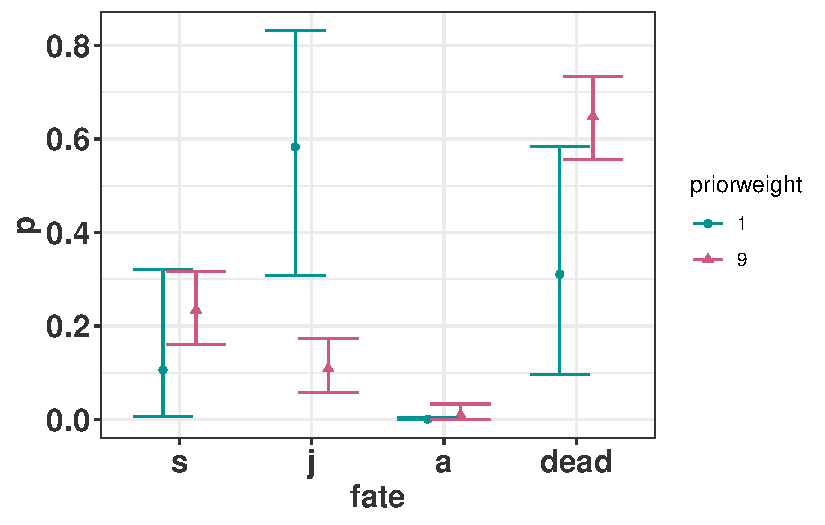
\includegraphics{108-Bayesian_PPM_files/figure-pdf/bayes16-1.pdf}

\begin{center}\rule{0.5\linewidth}{0.5pt}\end{center}

\section{\texorpdfstring{Intervalo de credibilidad para la tasa de
crecimiento asintótica
\(\lambda\)}{Intervalo de credibilidad para la tasa de crecimiento asintótica \textbackslash lambda}}\label{intervalo-de-credibilidad-para-la-tasa-de-crecimiento-asintuxf3tica-lambda}

Obtener intervalos de credibilidad para la tasa de crecimiento
asintótica, \(\lambda\), requiere simular matrices a partir de las
distribuciones posteriores. Estas simulaciones usualmente son
complicadas de hacer, por lo que hemos incorporado en el paquete la
función \texttt{raretrans::sim\_transitions()} para generar una lista de
matrices simuladas dada la matriz observada y las previas. En otras
palabras, esta función se calcula múltiples veces de las matrices de
transición y fertilidad basándose en los datos observados y en los
valores \emph{a priori} especificados pero variando los valores de los
parámetros de las distribuciones beta y gamma.

\subsection{Simulación de una matriz de
transición}\label{simulaciuxf3n-de-una-matriz-de-transiciuxf3n}

Siguiendo el marco bayesiano que hemos venido trabajando en este
capítulo es necesario especificar las previas de la fertilidad como una
matriz. Las celdas de la matriz de los estados en los que que no hay
reproducción deben ser \texttt{NA}, usando \emph{NA\_real\_} el cual es
un valor que no está presente pero podría aceptar valores con puntos
decimales. Nota que el valor \emph{a priori} de la fertilidad es 0.0001.

\begin{Shaded}
\begin{Highlighting}[]
\NormalTok{alpha }\OtherTok{\textless{}{-}} \FunctionTok{matrix}\NormalTok{(}\FunctionTok{c}\NormalTok{(}\ConstantTok{NA\_real\_}\NormalTok{, }\ConstantTok{NA\_real\_}\NormalTok{, }\FloatTok{1e{-}5}\NormalTok{,}
                  \ConstantTok{NA\_real\_}\NormalTok{, }\ConstantTok{NA\_real\_}\NormalTok{, }\ConstantTok{NA\_real\_}\NormalTok{,}
                  \ConstantTok{NA\_real\_}\NormalTok{, }\ConstantTok{NA\_real\_}\NormalTok{, }\ConstantTok{NA\_real\_}\NormalTok{), }\AttributeTok{nrow=}\DecValTok{3}\NormalTok{, }\AttributeTok{ncol =} \DecValTok{3}\NormalTok{, }\AttributeTok{byrow =} \ConstantTok{TRUE}\NormalTok{)}

\NormalTok{beta }\OtherTok{\textless{}{-}} \FunctionTok{matrix}\NormalTok{(}\FunctionTok{c}\NormalTok{(}\ConstantTok{NA\_real\_}\NormalTok{, }\ConstantTok{NA\_real\_}\NormalTok{, }\FloatTok{1e{-}5}\NormalTok{,}
                 \ConstantTok{NA\_real\_}\NormalTok{, }\ConstantTok{NA\_real\_}\NormalTok{, }\ConstantTok{NA\_real\_}\NormalTok{,}
                 \ConstantTok{NA\_real\_}\NormalTok{, }\ConstantTok{NA\_real\_}\NormalTok{, }\ConstantTok{NA\_real\_}\NormalTok{), }\AttributeTok{nrow=}\DecValTok{3}\NormalTok{, }\AttributeTok{ncol =} \DecValTok{3}\NormalTok{, }\AttributeTok{byrow =} \ConstantTok{TRUE}\NormalTok{)}

\FunctionTok{fill\_fertility}\NormalTok{(TF, N, }\AttributeTok{alpha =}\NormalTok{ alpha, }\AttributeTok{beta =}\NormalTok{ beta)}
\end{Highlighting}
\end{Shaded}

\begin{verbatim}
   
            s         j         a
  s 0.0000000 0.0000000 0.1176473
  j 0.0000000 0.0000000 0.0000000
  a 0.0000000 0.0000000 0.0000000
\end{verbatim}

El cambio en la fertilidad es \textless{} 0,0001 en comparación con el
valor observado.

\subsection{UNA simulación de la matriz de
transición}\label{una-simulaciuxf3n-de-la-matriz-de-transiciuxf3n}

Corra el script múltiples veces, y verá que los valores cambian en cada
simulación. En este script la simulación es solamente de una vez
(samples = 1). Este script es para que visualizan lo que hace la función
\texttt{sim\_transitions()}.

\begin{Shaded}
\begin{Highlighting}[]
\FunctionTok{sim\_transitions}\NormalTok{(}
\NormalTok{  TF,}
\NormalTok{  N,}
  \AttributeTok{P =}\NormalTok{ RLT\_Tprior,}
  \AttributeTok{alpha =}\NormalTok{ alpha,}
  \AttributeTok{beta =}\NormalTok{ beta,}
  \AttributeTok{priorweight =} \FloatTok{0.5}\NormalTok{,}
  \AttributeTok{samples =} \DecValTok{1}
\NormalTok{)}
\end{Highlighting}
\end{Shaded}

\begin{verbatim}
[[1]]
           [,1]        [,2]       [,3]
[1,] 0.20501852 0.007900161 0.20122316
[2,] 0.32072063 0.724291565 0.00125244
[3,] 0.01822617 0.197242890 0.95186855
\end{verbatim}

\subsection{Simulación de 5000 matrices de
transición}\label{simulaciuxf3n-de-5000-matrices-de-transiciuxf3n}

Ahora simulamos 5000 veces, calculamos el valor \(\lambda\) de cada
matriz y creamos un histograma de su distribución. Se añade los valores
de lambda en un objeto llamado RLT\_0.5. Se visualiza la distribución de
\(\lambda\) usando un histograma. Note que el valor de \(\lambda\) = 1
queda dentro de la distribución, en otras palabras el histograma muestra
que la mayoría de los valores de \(\lambda\) están cerca de 1.

\begin{Shaded}
\begin{Highlighting}[]
\CommentTok{\#set.seed(8390278) \# make this part reproducible}
\NormalTok{alpha2 }\OtherTok{\textless{}{-}} \FunctionTok{matrix}\NormalTok{(}\FunctionTok{c}\NormalTok{(}\ConstantTok{NA\_real\_}\NormalTok{, }\ConstantTok{NA\_real\_}\NormalTok{, }\FloatTok{0.025}\NormalTok{,}
                   \ConstantTok{NA\_real\_}\NormalTok{, }\ConstantTok{NA\_real\_}\NormalTok{, }\ConstantTok{NA\_real\_}\NormalTok{,}
                   \ConstantTok{NA\_real\_}\NormalTok{, }\ConstantTok{NA\_real\_}\NormalTok{, }\ConstantTok{NA\_real\_}\NormalTok{), }\AttributeTok{nrow=}\DecValTok{3}\NormalTok{, }\AttributeTok{ncol =} \DecValTok{3}\NormalTok{, }\AttributeTok{byrow =} \ConstantTok{TRUE}\NormalTok{)}

\NormalTok{beta2 }\OtherTok{\textless{}{-}} \FunctionTok{matrix}\NormalTok{(}\FunctionTok{c}\NormalTok{(}\ConstantTok{NA\_real\_}\NormalTok{, }\ConstantTok{NA\_real\_}\NormalTok{, }\DecValTok{1}\NormalTok{,}
                  \ConstantTok{NA\_real\_}\NormalTok{, }\ConstantTok{NA\_real\_}\NormalTok{, }\ConstantTok{NA\_real\_}\NormalTok{,}
                  \ConstantTok{NA\_real\_}\NormalTok{, }\ConstantTok{NA\_real\_}\NormalTok{, }\ConstantTok{NA\_real\_}\NormalTok{), }\AttributeTok{nrow=}\DecValTok{3}\NormalTok{, }\AttributeTok{ncol =} \DecValTok{3}\NormalTok{, }\AttributeTok{byrow =} \ConstantTok{TRUE}\NormalTok{)}

\CommentTok{\# generar 5000 matrices basado en las previas de transciones y de fertilidades, el tamaño de muestra, en adición de los datos}
\NormalTok{RLT\_0}\FloatTok{.5}\NormalTok{s }\OtherTok{\textless{}{-}} \FunctionTok{sim\_transitions}\NormalTok{(TF, N, }\AttributeTok{P =}\NormalTok{ RLT\_Tprior, }\AttributeTok{alpha =}\NormalTok{ alpha2, }\AttributeTok{beta =}\NormalTok{ beta2,}
                \AttributeTok{priorweight =} \FloatTok{0.5}\NormalTok{, }\AttributeTok{samples =} \DecValTok{5000}\NormalTok{)}


\CommentTok{\# extraer los valores de lambda de cada simulación en un histograma}

\NormalTok{RLT\_0}\FloatTok{.5} \OtherTok{\textless{}{-}} \FunctionTok{tibble}\NormalTok{(}\AttributeTok{lposterior =} \FunctionTok{map\_dbl}\NormalTok{(RLT\_0}\FloatTok{.5}\NormalTok{s, lambda)) }\CommentTok{\# convertir la lista en un tibble}
\FunctionTok{ggplot}\NormalTok{(}\AttributeTok{data =}\NormalTok{ RLT\_0}\FloatTok{.5}\NormalTok{,}
       \AttributeTok{mapping =} \FunctionTok{aes}\NormalTok{(}\AttributeTok{x =}\NormalTok{ lposterior)) }\SpecialCharTok{+} 
  \FunctionTok{geom\_histogram}\NormalTok{(}\AttributeTok{binwidth =} \FloatTok{0.01}\NormalTok{, }\AttributeTok{colour=}\StringTok{"white"}\NormalTok{) }\SpecialCharTok{+} 
  \FunctionTok{theme\_bw}\NormalTok{() }\SpecialCharTok{+}
  \FunctionTok{rlt\_style\_fill}\NormalTok{() }\SpecialCharTok{+}
  \FunctionTok{geom\_vline}\NormalTok{(}\AttributeTok{xintercept =} \DecValTok{1}\NormalTok{, }
                \AttributeTok{color =} \StringTok{"\#009392"}\NormalTok{, }\AttributeTok{linewidth=}\FloatTok{1.5}\NormalTok{)}
\end{Highlighting}
\end{Shaded}

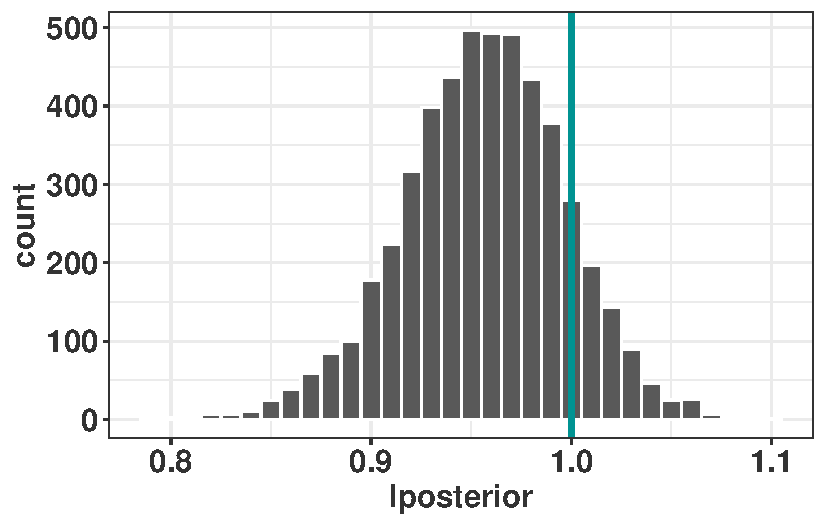
\includegraphics{108-Bayesian_PPM_files/figure-pdf/bayes19-1.pdf}

\begin{center}\rule{0.5\linewidth}{0.5pt}\end{center}

\section{\texorpdfstring{Determinar si el \(\lambda\) es
significativamente diferente de
1}{Determinar si el \textbackslash lambda es significativamente diferente de 1}}\label{determinar-si-el-lambda-es-significativamente-diferente-de-1}

Esta prueba está basada en la simulación de la distribución posterior.
Se calcula la distribución de las \(\lambda\) y se determina si
\(\lambda\) observada es significativamente más grande que 1. También
podemos calcular algunas estadísticas descriptivos, donde
\texttt{p\_increase} es el probabilidad de que \(\lambda > 1\). En este
caso el valor de \(\lambda\) no es significativamente más grande que 1
ya que se obtuvo un valor de 0.14. Aunque el histograma sugiere que el
crecimiento es menor de 1, la probabilidad de que \(\lambda\) sea mayor
que 1 es de 0.14, lo que indica que hay una probabilidad del 14\% de que
la población esté creciendo. Dando poca apoyo que la población este
creciendo.

\begin{Shaded}
\begin{Highlighting}[]
\NormalTok{RLT\_0}\FloatTok{.5}\NormalTok{\_summary }\OtherTok{\textless{}{-}} \FunctionTok{summarize}\NormalTok{(}
\NormalTok{  RLT\_0}\FloatTok{.5}\NormalTok{,}
  \AttributeTok{medianaL =} \FunctionTok{median}\NormalTok{(lposterior),}
  \AttributeTok{promedioL =} \FunctionTok{mean}\NormalTok{(lposterior),}
  \AttributeTok{skewnessL=}\NormalTok{e1071}\SpecialCharTok{::}\FunctionTok{skewness}\NormalTok{(lposterior, }\AttributeTok{type=}\DecValTok{2}\NormalTok{),}
  \AttributeTok{ICrBajo =} \FunctionTok{quantile}\NormalTok{(lposterior, }\AttributeTok{probs =} \FloatTok{0.025}\NormalTok{),}
  \AttributeTok{ICrAlto =} \FunctionTok{quantile}\NormalTok{(lposterior, }\AttributeTok{probs =} \FloatTok{0.975}\NormalTok{),}
  \AttributeTok{p\_increase =} \FunctionTok{sum}\NormalTok{(lposterior }\SpecialCharTok{\textgreater{}} \FloatTok{1.}\NormalTok{) }\SpecialCharTok{/} \FunctionTok{n}\NormalTok{()}
\NormalTok{)}
\end{Highlighting}
\end{Shaded}

\subsection{Tabla de resultado de
lambda}\label{tabla-de-resultado-de-lambda}

\begin{Shaded}
\begin{Highlighting}[]
\NormalTok{gt}\SpecialCharTok{::}\FunctionTok{gt}\NormalTok{(}\FunctionTok{signif}\NormalTok{(RLT\_0}\FloatTok{.5}\NormalTok{\_summary, }\AttributeTok{digits =} \DecValTok{2}\NormalTok{))}
\end{Highlighting}
\end{Shaded}

\begin{table}
\fontsize{12.0pt}{14.0pt}\selectfont
\begin{tabular*}{\linewidth}{@{\extracolsep{\fill}}rrrrrr}
\toprule
medianaL & promedioL & skewnessL & ICrBajo & ICrAlto & p\_increase \\ 
\midrule\addlinespace[2.5pt]
0.96 & 0.96 & -0.13 & 0.88 & 1 & 0.15 \\ 
\bottomrule
\end{tabular*}
\end{table}

\begin{center}\rule{0.5\linewidth}{0.5pt}\end{center}

\section{ADDENDUM}\label{addendum}

\subsection{Uso de previas uniformes}\label{uso-de-previas-uniformes}

En esta sección es para demostrar porque no es recomendable el uso de
distribuciones previas uniformes. Si se entiende el concepto de valores
\emph{a priori} y \emph{a posteriori} no es necesario leer esta sección.

\subsection{Matriz de transición}\label{matriz-de-transiciuxf3n}

A continuación vamos a añadir una distribución Dirichlet uniforme como
previa con un peso = \(1\) a la matriz de transición, \(T\). En este
caso, tenemos 4 destinos (3 + muerte), por lo que cada destino añade
0.25 a la matriz de destinos \emph{observados} (¡no a la matriz de
transición!). Cuando especificamos una matriz con valores \emph{a
priori} para las transiciones, hay una fila más que columnas. Esta fila
extra representa la mortalidad por etapa.

Note que no se recomienda el uso de una previa uniforme, aquí se utiliza
sólo para mostrar el concepto. Una distribución previa uniforme no
refleja un ciclo de vida razonable para especie biológicas. Por ejemplo,
una previa uniforme podría hacer que las plántulas pasen a adulto de un
tiempo a otro o que los adultos regresen a ser plántulas, lo cual no
tiene mucho sentido biológico en muchas especies. Considera lo siguiente
¿es posible que una ballena beba pueda pasar a ser madre el siguiente
año? Añadir una transición de 0.25 de ballena bebé a madre no tiene
sentido biológico.

Note que ahora la matriz de transición es ergódica pero no tiene sentido
biológico. Compare la matriz con las previas uniformes versus la matriz
original.

\begin{Shaded}
\begin{Highlighting}[]
\NormalTok{Tprior }\OtherTok{\textless{}{-}} \FunctionTok{matrix}\NormalTok{(}\FloatTok{0.25}\NormalTok{, }\AttributeTok{byrow =} \ConstantTok{TRUE}\NormalTok{, }\AttributeTok{ncol =} \DecValTok{3}\NormalTok{, }\AttributeTok{nrow =} \DecValTok{4}\NormalTok{) }\CommentTok{\# crear la matriz de previas uniformes}

\NormalTok{Tprior}
\end{Highlighting}
\end{Shaded}

\begin{verbatim}
     [,1] [,2] [,3]
[1,] 0.25 0.25 0.25
[2,] 0.25 0.25 0.25
[3,] 0.25 0.25 0.25
[4,] 0.25 0.25 0.25
\end{verbatim}

\begin{Shaded}
\begin{Highlighting}[]
\NormalTok{Posterior\_con\_Unif }\OtherTok{=} \FunctionTok{fill\_transitions}\NormalTok{(TF, N, }\AttributeTok{P =}\NormalTok{ Tprior) }\CommentTok{\# resultado de la matriz de transición básica con las previas}

\NormalTok{Posterior\_con\_Unif}
\end{Highlighting}
\end{Shaded}

\begin{verbatim}
           [,1]        [,2]        [,3]
[1,] 0.10416667 0.005208333 0.007142857
[2,] 0.60416667 0.567708333 0.007142857
[3,] 0.02083333 0.296875000 0.835714286
\end{verbatim}

\begin{Shaded}
\begin{Highlighting}[]
\CommentTok{\# Para entender las diferencias del impacto de las matriz compara los resultados con *$T* del objeto *TF*}
\NormalTok{TF}
\end{Highlighting}
\end{Shaded}

\begin{verbatim}
$T
   
             s          j          a
  s 0.09090909 0.00000000 0.00000000
  j 0.63636364 0.57446809 0.00000000
  a 0.00000000 0.29787234 0.85294118

$F
   
            s         j         a
  s 0.0000000 0.0000000 0.1176471
  j 0.0000000 0.0000000 0.0000000
  a 0.0000000 0.0000000 0.0000000
\end{verbatim}

\begin{center}\rule{0.5\linewidth}{0.5pt}\end{center}

\subsection{¿Cómo calcular en forma directa las transiciones de estado
?}\label{cuxf3mo-calcular-en-forma-directa-las-transiciones-de-estado}

Podemos obtener el resultado haciendo los cálculos directamente. Lo
primero que necesitamos es el vector de observaciones porque la
distribución posterior se calcula a partir de las observaciones de
transiciones, no de la matriz de transiciones. Si no tiene experiencia
con análisis Bayesiano es recomendable seguir los siguientes scripts

\begin{Shaded}
\begin{Highlighting}[]
\NormalTok{Tobs }\OtherTok{\textless{}{-}} \FunctionTok{sweep}\NormalTok{(TF}\SpecialCharTok{$}\NormalTok{T, }\DecValTok{2}\NormalTok{, N, }\StringTok{"*"}\NormalTok{) }\CommentTok{\# obtener las observaciones de transiciones}
\NormalTok{Tobs }\OtherTok{\textless{}{-}} \FunctionTok{rbind}\NormalTok{(Tobs, N }\SpecialCharTok{{-}} \FunctionTok{colSums}\NormalTok{(Tobs)) }\CommentTok{\# añadir la fila de muerte}
\NormalTok{Tobs }\OtherTok{\textless{}{-}}\NormalTok{ Tobs }\SpecialCharTok{+} \FloatTok{0.25} \CommentTok{\# añadir los valores de las previas}
\FunctionTok{sweep}\NormalTok{(Tobs, }\DecValTok{2}\NormalTok{, }\FunctionTok{colSums}\NormalTok{(Tobs), }\StringTok{"/"}\NormalTok{)[}\SpecialCharTok{{-}}\DecValTok{4}\NormalTok{, ] }\CommentTok{\# dividir por la suma de la columna y descarta la fila de muerte}
\end{Highlighting}
\end{Shaded}

\begin{verbatim}
           s           j           a
s 0.10416667 0.005208333 0.007142857
j 0.60416667 0.567708333 0.007142857
a 0.02083333 0.296875000 0.835714286
\end{verbatim}

La previa uniforme ``rellena'' las transiciones faltantes, pero también
crea problemas porque algunos de los valores de transición que se asigna
son biológicamente imposibles en muchas especies. Por ejemplo, para la
transición de adulto a plántula se asigna un valor, sin embargo, este
valor sólo es posible en la matriz de fertilidad \(F\) en las especies
de \emph{Lepanthes}. Debido a esto, no es recomendable el uso de previas
uniformes ya que NO toma en cuenta el ciclo de vida de nuestra especie.
Sera necesario crear una matriz de \textbf{priors} que refleje el ciclo
de vida de la especie de interés.

\begin{center}\rule{0.5\linewidth}{0.5pt}\end{center}

Revisión RLT:

Sept 15, 2024

RLT: Oct 8, 2024

Paola: Apr 25, 2025

RLT: May 27, 2025

\phantomsection\label{refs}
\begin{CSLReferences}{1}{0}
\bibitem[\citeproctext]{ref-tremblay2021population}
Tremblay R, Tyre AJ, Pérez M-E, Ackerman JD. 2021. Population
projections from holey matrices: Using prior information to estimate
rare transition events. \emph{Ecological Modelling} 447:109526.

\bibitem[\citeproctext]{ref-raretrans2024}
Tyre A, Tremblay R, Perez M. 2024.
\emph{\href{https://github.com/atyre2/raretrans}{Raretrans: Bayesian
priors for matrix population models}}.

\end{CSLReferences}


\backmatter


\end{document}
